\documentclass[a4paper]{article}

\usepackage{array}
\usepackage[
    style=apa, 
    backend=biber, 
    sorting=none
]{biblatex}
\usepackage{graphicx}
\usepackage{enumitem}
\usepackage{geometry}
\usepackage{sectsty}
\usepackage{indentfirst}
\usepackage{times}
\usepackage{listings}
\usepackage{longtable}
\usepackage{setspace}
\usepackage[colorlinks=true,linkcolor=black,anchorcolor=black,citecolor=black,filecolor=black,menucolor=black,runcolor=black,urlcolor=black]{hyperref}

\setlist{
  listparindent=\parindent,
  parsep=0pt,
}

% code block style
% -- Defining colors:
\usepackage[dvipsnames]{xcolor}
\definecolor{codegreen}{rgb}{0,0.6,0}
\definecolor{codegray}{rgb}{0.5,0.5,0.5}
\definecolor{codepurple}{rgb}{0.58,0,0.82}
\definecolor{backcolour}{rgb}{0.95,0.95,0.92}% Definig a custom style:
\lstdefinestyle{mystyle}{
    backgroundcolor=\color{backcolour},   
    commentstyle=\color{codepurple},
    keywordstyle=\color{NavyBlue},
    numberstyle=\tiny\color{codegray},
    stringstyle=\color{codepurple},
    basicstyle=\ttfamily\footnotesize\bfseries,
    breakatwhitespace=false,         
    breaklines=true,                 
    captionpos=t,                    
    keepspaces=true,                 
    numbers=left,                    
    numbersep=5pt,                  
    showspaces=false,                
    showstringspaces=false,
    showtabs=false,                  
    tabsize=2
}% -- Setting up the custom style:
\lstset{style=mystyle}

\sectionfont{\centering}
\addbibresource{citation/citation.bib}
\addbibresource{citation/aldih.bib}
\graphicspath{{./images/}}
\geometry{a4paper, top=4.0cm, bottom=3.0cm,
          left=4.0cm, includehead, includefoot}
\renewcommand\contentsname{Daftar Pustaka}
\emergencystretch=2em

% bab command
\newcommand{\bab}[1]{%
    \section*{#1}%
    \addcontentsline{toc}{section}{\protect\numberline{}#1}%
}

\newcommand{\subbab}[1]{%
    \subsection*{#1}%
    \addcontentsline{toc}{subsection}{\protect\numberline{}#1}%
}

\newcommand{\subsubbab}[1]{%
    \subsubsection*{#1}%
    \addcontentsline{toc}{subsubsection}{\protect\numberline{}#1}%
}

\begin{document}
\setstretch{1.5}

\title{SKRIPSI NON KELAS\\Shumishumi - Online Marketplace For Hobby With Interest Level Filtering and Recommendation System Using Knowledge Graph Implementation\large\\\textbf{Topic: }\textit{E-Application}}
\author{2301862632 - Aldih Suhandi - \textit{Computer Science} / 082122704561\\2301872596 - Chandra Wijaya - \textit{Computer Science} / 081287588816\\2301867324 - Ibrahim Seto Aditama - \textit{Computer Science} / 081213423549}
\maketitle
\begin{figure}[h]
    \centering
    
\includegraphics[width=8cm,height=4cm]{logo_binus.png}\\
    Binus University Alam Sutera\\
    2023
\end{figure}
\begin{figure}[h]
    \centering
    Diperiksa Oleh**\\
    \begin{tabular}{@{}p{2in}@{}}
        \centering
        
\includegraphics[width=3cm]{ttd.png} \\
        D5186 - Pualam Dipa Nusantara
    \end{tabular}
\end{figure}

\newpage
\addcontentsline{toc}{section}{\protect\numberline{}Daftar Pustaka}
\tableofcontents

\newpage
\bab{Bab 1. Pendahuluan}

\subbab{1.1 Latar Belakang}

Hobi dapat diartikan sebagai suatu aktivitas yang dilakukan dalam waktu luang dengan tujuan untuk mendapatkan rasa kebahagiaan. Hobi ini juga dapat menjadi distraksi dari rasa gelisah yang dimiliki atau dialami oleh seseorang. Hobi juga dapat memberi rasa tujuan hidup kepada seseorang, terutama ketika hobi tersebut dapat dilakukan bersama-sama dengan sebuah kelompok yang memiliki minat hobi yang sejenis\autocite{zaidi2022passion}.

Tidak semua hobi dapat dilakukan dengan mudahnya tanpa memerlukan barang-barang tertentu yang khusus digunakan untuk menjalankan aktivitas hobi tersebut. Seperti contoh, bagi seseorang yang memiliki hobi memancing, orang tersebut harus memiliki alat pemancing ikan untuk bisa melakukan aktivitas tersebut. Contoh lainnya adalah orang-orang yang memiliki hobi bermain bulu tangkis (\textit{badminton}), mereka harus mempunyai raket \textit{badminton} terlebih dahulu agar bisa menjalankan hobi tersebut. Maka dari itu, barang-barang tersebut perlu dicari dan didapatkan terlebih dahulu. Caranya adalah dengan mendatangi toko yang menjual barang-barang tersebut atau membeli barang tersebut secara \textit{online} melalui \textbf{internet}.

Internet merupakan hasil dari perkembangan teknologi yang memiliki dampak cukup tinggi, yang dimana di Indonesia sendiri, internet mendapatkan peningkatan popularitas yang cukup drastis. Hal ini dapat diukur dengan melihat peningkatan pengguna internet tersebut di setiap tahunnya. Menurut survey yang diadakan oleh Asosiasi Penyelenggara Jasa Internet Indonesia (APJII) di tahun 2017, perkembangan pengguna internet di Indonesia dari tahun 2016 ke tahun 2017 sendiri memiliki pertambahan sebesar 10.56 juta, yakni dari 132.7 juta pengguna di tahun 2016 ke 143.26 juta pada tahun 2017\autocite{indonesia2017infografis}.

Dari kegiatan penggunaan internet yang ada, aktivitas usaha jual beli barang yang dilakukan secara \textit{text/chatting} ataupun melalui \textit{e-commerce} merupakan kegiatan yang cukup populer dilakukan melalui internet. Dimana di Indonesia sendiri berdasarkan survei yang dilakukan oleh APJII, proses pembelian barang mencakupi 32.19\% dan penjualan barang sebesar 8.12\% pada layanan yang diakses ketika menggunakan internet\autocite{indonesia2017infografis}. \textit{Platform} yang digunakan untuk mempermudah usaha kegiatan jual beli barang biasanya dilengkapi dengan fitur pencarian/\textit{searching} yang cukup cepat, dimana barang dapat dicari dan ditemukan melalui pencarian namanya ataupun menelusuri kategori dari barang tersebut. Kegiatan jual-beli barang ini mencakupi kebutuhan bahan baku hingga kebutuhan-kebutuhan tambahan lainnya.

Salah satu tempat dimana kegiatan jual beli tersebut berlangsung adalah dalam sebuah \textit{Web Application} atau aplikasi web, yang dimana aplikasi web itu sendiri adalah sebuah program aplikasi yang di simpan di sebuah \textit{remote server} dan dapat diakses dengan \textit{web browser} melalui internet\autocite{what-is-web-app}. Pada umumnya, barang-barang kebutuhan hobi diperjualbelikan di dalam \textit{e-commerce} atau sebuah \textit{online marketplace}. Disana, barang kebutuhan hobi dijual bersamaan dengan barang-barang lain yang tidak berhubungan sama sekali dengan suatu hobi. Adapun barang kebutuhan hobi dijual ke sebuah \textit{online marketplace} yang hanya terfokus kepada hobi tertentu saja. Jenis \textit{online marketplace} ini biasa disebut dengan istilah \textit{hobby shop}. 

Alasan utama mengapa penelitian ini memilih topik yang berfokus pada kegiatan jual beli barang kebutuhan hobi adalah dikarenakannya tingginya peningkatan kegiatan jual beli di pasar kebutuhan barang hobi semenjak pandemi COVID-19 kemarin. Pandemi COVID-19 yang melanda dunia selama kurang lebih dua setengah tahun lamanya itu, membuat banyak orang mengalamai kebosanan dikarenakan adanya \textit{lockdown} dan aturan-aturan \textit{social distancing} ketat yang membuat aktivitas masyarakat menjadi sangat terbatas\autocite{boredom-in-covid-19-pandemic}. Semenjak itulah, banyak orang yang kembali menjalankan kegiatan hobi lama mereka atau bahkan mencari kegiatan lain yang dapat dijadikan hobi baru untuk mengisi waktu luang mereka di masa pandemi tersebut. Hal ini mengakibatkan pasar yang berfokus pada bidang jual beli barang kebutuhan hobi meningkat drastis. 

Contohnya dapat dilihat dari salah satu rantai ritel \textit{superstore} yang bergerak di bidang hobi di segi seni dan kerajinan dari Inggris yang bernama \textbf{Hobbycraft}. Mereka melaporkan bahwa pada tahun dimana pandemi COVID-19 sedang merajalela, mereka kedatangan banyak pengguna baru yang berjumlah kurang lebih sebanyak 1.3 juta akun, yang sebagian besarnya adalah para pengguna dari kaum \textit{millenial}\autocite{hobbycraft-fast-online-growth}. Bukti lainnya juga dapat dilihat dari salah satu \textit{e-commerce} terbesar di Indonesia yakni \textbf{Tokopedia} yang melaporkan bahwa hasil penjualan dari transaksi barang-barang yang berhubungan dengan kebutuhan \textbf{hobi} meningkat drastis di masa pandemi COVID-19. Mulai dari hobi olahraga, membaca buku, seni hingga memasak\autocite{tokped-hobbies-goods-sales-increased}.

Alasan lain mengapa topik ini dipilih adalah karena kurangnya jumlah \textit{online hobby shop} yang menjual barang kebutuhan untuk berbagai macam hobi. Kebanyakan dari \textit{hobby shop} yang ada (terutama di Indonesia) hanya berfokus pada satu hobi yang spesifik saja. Salah satu yang cukup terkenal adalah \textbf{Kyou Hobby Shop} atau biasa disebut sebagai \textbf{KyouID}. \textbf{KyouID} merupakan sebuah \textit{hobby shop} yang menjual berbagai jenis produk khusus untuk orang-orang yang hobi mengoleksi produk atau \textit{merchandise} yang berhubungan erat dengan kebudayaan \textit{anime} dari Jepang. Contoh produk yang mereka jual dapat berupa \textit{figurine}/miniatur karakter, stiker dari sebuah karakter, poster seni dan berbagai macam \textit{merchandise} lainnya yang berhubungan dengan satu hobi tersebut. 

Maka dari itu, penelitian ini mengusulkan untuk membuat sebuah aplikasi berbasis \textit{web} yang lebih terfokus ke arah produk-produk kebutuhan hobi dibandingkan dengan \textit{e-commerce} atau \textit{marketplace}. Namun, cakupan aplikasi \textit{web} ini lebih terfokus ke arah kebutuhan hobi yang lebih luas. Aplikasi \textit{web} ini mencakupi berbagai macam jenis hobi yang lebih banyak apabila dibandingkan dengan \textit{hobby shop} yang hanya terfokus pada satu jenis hobi saja. Para pengguna dapat mencari dan memilih berbagai macam produk untuk hobi yang berbeda-beda.

Untuk memulai sebuah hobi baru, terkadang juga muncul suatu permasalahan baru, yakni kebingungan atau merasa ragu untuk mencari produk yang cocok sebagai titik mulai untuk menjalankan hobi tersebut. Begitu juga dengan para pengguna yang sudah berpengalaman pada hobi tertentu. Terkadang, mereka juga mengalami kesulitan untuk mencari suatu produk yang dapat mendukung kegiatan hobi mereka yang cukup ekstrim atau yang dapat mendukung kegiatan hobi mereka dalam jangka waktu yang lama. Seperti contoh, seseorang yang hobi bersepeda di pegunungan membutuhkan sebuah sepeda yang kokoh dan aman untuk melewati rintangan yang cukup berat di wilayah pegunungan tersebut. Untuk itu, penelitian ini melakukan sebuah survei untuk mengumpulkan pendapat dari para pengguna mengenai tingkat kesulitan untuk mendapatkan barang-barang hobi yang diinginkan. Salah satu dari pertanyaan dalam survei tersebut adalah \textit{"Apakah anda takut untuk mengambil hobi baru karena tidak tahu mulai dari mana?”}, pertanyaan ini mendapatkan respon sebesar 66.7\% yang menjawab \textit{"iya"}. Pada pertanyaan yang berhubungan mengenai kesulitan untuk memilih barang yang cocok memiliki respons \textit{"iya"} sebanyak diatas 50\%. Tingkat jawaban \textit{"iya"} yang tinggi pada kedua pertanyaan tersebut menunjukkan bahwa tingkat kesulitan untuk mencari barang kebutuhan hobi memang cukup tinggi. Untuk menyelesaikan permasalahan tersebut, aplikasi ini akan mengimplementasikan sebuah fitur utama yang cukup unik dan cocok digunakan pada aplikasi \textit{web} jual beli barang kebutuhan hobi.

Fitur utama tersebut berbentuk sebuah dua penilaian tingkat peminatan pada suatu barang kebutuhan hobi sebagai sebuah sistem saring tambahan untuk mencari barang tersebut yang diberi nama \textit{Interest Level Filtering}. Penilaian tersebut diberikan oleh penjual barang tersebut dan nantinya juga dapat diberi oleh pembeli sebagai validasi apakah penilaian yang diberikan oleh penjual tersebut sesuai dengan tingkat minat hobinya atau tidak. Fitur ini dibuat dengan tujuan untuk membantu meningkatkan keyakinan pengguna untuk memilih barang kebutuhan hobi yang sesuai dengan hobi yang dilakukannya, dari yang ingin memulai suatu hobi baru maupun yang ingin mencari barang-barang kebutuhan hobi yang sudah bertingkat antusias atau yang sudah berpengalaman.

Contoh kasus penggunaan fitur \textit{Interest Level} tersebut adalah seperti berikut, misal untuk hobi bermain gitar. Apabila seorang pengguna baru saja menjalani hobi tersebut atau baru saja belajar bermain gitar, tentunya gitar yang cocok untuk memulai belajar adalah sebuah gitar akustik biasa. Maka dari itu, untuk sebuah produk berupa gitar akustik biasa ('biasa' disini berarti yang berstandar rata-rata atau bukan yang bermerek terkenal dan mahal) akan diberikan penilaian setara dengan "\textit{Beginner}" atau "Pemula" oleh penjual dari barang tersebut. Dan penilaian dari penjual tersebut dapat di nilai kembali oleh pembeli setelah membeli produk tersebut. Penilaian dari pembeli itu dapat digunakan sebagai validasi apakah penilaian tersebut cocok dengan barang yang dijualnya, dan begitu seterusnya untuk produk-produk kebutuhan hobi lainnya.

Fitur utama lain yang akan dikembangkan pada penelitian ini selain dari fitur \textit{Interest Level} diatas adalah sebuah sistem rekomendasi (\textit{Recommendation System}). Sistem rekomendasi ini akan diimplementasikan pada halaman utama aplikasi \textit{web} ini. Sistem rekomendasi inilah yang akan membantu memberikan saran kepada pengguna terhadap produk-produk yang paling relevan bagi pengguna tersebut. Sistem rekomendasi ini bekerja berdasarkan seberapa banyakkah barang-barang kebutuhan hobi tertentu yang telah pengguna tersebut cari atau lihat selama menggunakan aplikasi \textit{web} Shumishumi.

Aplikasi ini juga memiliki sebuah satu fitur pendukung, yakni sebuah tempat atau wadah untuk melakukan diskusi (layaknya sebuah forum diskusi). Proses diskusi ini dapat dilakukan melalui sebuah postingan yang di\textit{post} pada kategori hobi masing-masing sesuai dengan minat hobinya. Tujuan dari fitur ini adalah agar para pengguna yang tertarik dengan hobi tersebut dapat saling berdiskusi atau berinteraksi secara \textit{online} untuk membahas berbagai macam jenis barang yang cocok dengan hobi yang mereka minati tersebut.

Tentunya aplikasi \textit{online marketplace} seperti yang dikerjakan pada penelitian ini bukanlah yang pertama kali dibuat atau dikembangkan. Ada beberapa penelitian terdahulu yang juga telah mencoba dan/atau berhasil membuat aplikasi berjenis \textit{marketplace} dengan fitur dan tujuannya yang berbeda antara satu dengan yang lain. Beberapa aplikasi \textit{marketplace} sejenis tersebut dapat dibandingkan dengan aplikasi yang akan dikerjakan pada penelitian ini. Seperti aplikasi pada penelitian yang dilakukan oleh Heru Nugroho dengan rekan-rekannya yaitu sebuah aplikasi \textit{marketplace} berbasis \textit{mobile} yang menjual belikan produk-produk agrikultur. Aplikasi tersebut bertujuan untuk mempermudah para petani atau pekebun untuk menjual belikan produk agrikultur mereka ke masyarakat umum\autocite{agriculture-marketplace}. Selain dari sektor agrikultur, terdapat juga penelitian yang membuat aplikasi sejenis, namun pada sektor perikanan. Yaitu, penelitian yang dilakukan oleh Mohammad Nazrul bersama dengan rekan-rekannya yang membuat aplikasi \textit{marketplace} berbasis \textit{mobile} yang menjual belikan ikan\autocite{fishes-marketplace}. Lalu, pada ruang lingkup yang sama, ada sebuah penelitian yang dilakukan oleh Dwi bersama dengan rekan-rekannya yang membuat aplikasi jual beli ikan menggunakan metode \textit{SMS Gateway}\autocite{c2c-fish-marketplace}. Selanjutnya, penelitian yang dilakukan oleh N F Rozi dan rekan-rekannya dengan membuat aplikasi berbasis \textit{web} bernama \textbf{LIDI} yang ditujukkan sebagai tempat rental mobil secara \textit{online}\autocite{lidi-car-rental}. Terakhir, penelitian yang dilakukan oleh Rachmadita dan rekan-rekannya yang membuat sebuah aplikasi \textit{marketplace} yang menggabungkan usaha mikro, kecil dan menengah ke dalam satu \textit{platform} yang sama secara \textit{online} menggunakan metode \textit{Rapid Application Development}. Penelitian ini ditujukkan kepada Badan Usaha Milik Desa \textbf{(BUM)} di wilayah Desa Mekarsari, Bandung, Jawa Barat\autocite{bum-mekarsari}. Terakhir, ada dua aplikasi terkenal berbasis \textit{web} yang juga dapat dibandingkan dengan aplikasi yang akan dibuat pada proyek ini, yaitu satu aplikasi \textit{marketplace hobby shop} bernama \textbf{KyouID} dan aplikasi forum diskusi bernama \textbf{Reddit}.

Berdasarkan gambaran dan penjelasan serta data-data yang telah dikumpulkan diatas, dapat disimpulkan bahwa adanya peningkatan aktivitas jual beli barang melalui internet yang begitu besar (dari barang kebutuhan hobi maupun tidak) dalam beberapa tahun belakangan ini. Ditambah lagi dengan kesulitannya untuk memulai sebuah kegiatan hobi karena tidak yakin atas barang yang cocok sebagai titik awal untuk memulainya. Maka dari itu, proyek yang dikerjakan ini bermaksud untuk merancang dan membuat sebuah aplikasi berbasis \textit{web} yang berfokus pada kegiatan jual beli barang kebutuhan hobi apa saja tanpa merujuk pada satu atau beberapa hobi yang spesifik. Aplikasi ini diberi nama \textbf{ShumiShumi}. Aplikasi ini memiliki dua fitur utama dan satu fitur pendukung. Fitur utama pertama adalah \textit{Interest Level Filtering} yang merupakan sebuah sistem saring tambahan yang bekerja berdasarkan penilaian tingkat minat hobi yang diberikan oleh sisi penjual dan pembeli. Fitur kedua adalah sistem rekomendasi. Layaknya sistem rekomendasi pada umumnya, sistem ini yang akan menampilkan produk-produk paling relevan terhadap penggunanya. Fitur terakhir yang juga merupakan fitur pendukung dari aplikasi ini adalah sebuah tempat atau wadah untuk melakukan diskusi bagi para pengguna. Disini, para pengguna dapat berdiskusi untuk membahas mengenai barang-barang kebutuhan yang sesuai dengan hobinya masing-masing.


\subbab{1.2 Rumusan Masalah}

Sesuai dengan latar belakang yang telah dibahas di atas, rumusan masalah yang akan dikaji dalam proyek ini dapat dirangkum menjadi beberapa poin sebagai berikut:
\begin{enumerate}
    \item Bagaimana merancang sebuah aplikasi \textit{marketplace} hobi yang dapat membantu pelanggan atau \textit{user} dalam mencari barang hobi yang tepat
    \item Bagaimana merancang sebuah aplikasi \textit{marketplace} hobi yang dapat membantu penjual atau \textit{seller} dalam mengiklankan barang hobi yang mereka jual
    \item Bagaimana merancang fitur \textit{interest level} untuk membantu pencarian barang hobi yang tepat
    \item Bagaimana merancang fitur utama sistem rekomendasi untuk membantu penjual mengiklankan barangnya dengan rekomendasi barang hobi ke \textit{user} yang tepat
\end{enumerate}

\subbab{1.3 Ruang Lingkup}
Ruang lingkup dari proyek ini adalah perancangan sebuah aplikasi \textit{marketplace} terfokus untuk hobi dengan fitur utama sebuah filter terhadap tingkat kemahiran sebuah hobi, untuk menghindari pembahasan dan implementasi yang meluas dan supaya lebih terfokus maka ditetapkan batasan-batasan atau ruang lingkup sebagai berikut:
\begin{enumerate}
    \item Aplikasi hanya berbasis dan berada dalam bentuk aplikasi \textit{website}.
    \item Fitur utama untuk aplikasi ini adalah filter tingkat kemahiran dan  sistem rekomendasi.
    \item Integrasi dengan \textit{Midtrans} dan \textit{Xendit} sebagai \textit{payment gateway} yang akan digunakan.
    \item Dalam membangun \textit{Front-End} bahasa yang digunakan adalah \textit{Javascript} dan \textit{Framework} yang digunakkan adalah \textit{NextJs} versi 13.
    \item Dalam membuat tampilan aplikasi menggunakan \textit{html}, \textit{css} dan dengan dibantu sebuah \textit{CSS framework}, \textit{Tailwind} versi 3.2.7.
    \item Dalam membangun \textit{Back-End} bahasa yang digunakan adalah \textit{Java} dan menggunakkan \textit{Spring Framework} versi 2.7.6.
    \item \textit{Database} yang dipakai adalah \textit{mysql} versi 8.2.4-2.
\end{enumerate}

\subbab{1.4 Tujuan dan Manfaat}

Tujuan dari proyek ini adalah untuk merancang dan membuat sebuah aplikasi \textit{marketplace} yang berbasis \textit{web}. Tujuan secara khusus dapat ditulis sebagai poin sebagai berikut:
\begin{enumerate}
    \item Merancang dan membuat sebuah aplikasi \textit{marketplace} hobi yang dapat membantu pelanggan atau \textit{user} dalam mencari barang hobi yang tepat
    \item Merancang dan membuat sebuah aplikasi \textit{marketplace} hobi yang dapat membantu penjual atau \textit{seller} dalam mengiklankan barang hobi yang mereka jual
    \item Merancang dan membuat fitur \textit{interest level} untuk membantu pencarian barang hobi yang tepat
    \item Merancang dan membuat fitur utama sistem rekomendasi untuk membantu penjual mengiklankan barangnya dengan rekomendasi barang hobi ke \textit{user} yang tepat
\end{enumerate}

Manfaat yang diharapkan dari proyek ini adalah:
\begin{enumerate}
    \item Memberikan opsi untuk tempat \textit{marketplace} hobi
    \item Memberikan fitur yang berguna bagi pengguna dalam mencari barang yang tepat untuk mendukung hobi mereka sesuai dengan tingkat peminatan dan kemahiran mereka.
    \item Menyediakan tempat jual beli yang tepat untuk penjual barang hobi, dimana dengan sistem rekomendasi barang dibantu didorong atau disarankan ke pengguna yang tepat.
\end{enumerate}

\subbab{1.5 Metode Penelitian}

Metode Penelitian yang digunakkan adalah metode penelitian kualitatif, yang bersifat deskriptif dengan melakukan analisis\autocite{pengajar-kualitatif}, dan akan melakukan analisis dari hasil pengumpulan data yang dilakukan.


Pengumpulan data yang dilakukan adalah dengan membuat form survei menggunakan \textit{Google Form} untuk mendapatkan pendapat atas pertanyaan-pertanyaan yang terkait dengan alasan dari pembuatan aplikasi pada proyek ini. Dari hal mengenai pembelian barang hobi hingga tingkat kesulitan dalam menemukan barang yang cocok. Dari semua jawaban survei yang dikumpulkan tersebutlah, dapat memperoleh gambaran dan konfirmasi atas fitur-fitur yang proyek ini butuhkan.

\subbab{1.6 Sistematika Penulisan}
\textit{\textbf{Bab 1: Pendahuluan}} \newline
Bab pertama ini akan menjelaskan tentang latar belakang, rumusan masalah, tujuan, manfaat, ruang lingkup, dan metode penelitian yang dilakukan didalam proyek ini.

\textit{\textbf{Bab 2: Tinjauan Referensi}}\newline
Bab kedua menjelaskan tentang teori-teori yang digunakan sebagai acuan saat melakukan pembahasan masalah, menyimpulkan masalah tersebut menjadi \textit{requirement - requirement} yang bisa dijadikan pacuan saat membuat fitur dari aplikasi ini, dan hal-hal yang digunakan saat proses penulisan kode dan pengetesan fitur.

\textit{\textbf{Bab 3: Metode Penelitian}}\newline
Bab ketiga ini menjelaskan konsep metode penelitian yang dipakai dan alasan kenapa metode penelitian ini yang dipakai, selain itu disini menjelaskan tentang data - data yang dapat dikumpulkan dari hasil penelitian tersebut dan apa yang dapat disimpulkan.

\textit{\textbf{Bab 4: Hasil dan Pembahasan}}\newline
Bab keempat ini menjelaskan hasil penelitian dan pembahasan. Hasil penelitian yang telah dilakukan meliputi gambaran umum bagaimana \textit{software} yang dibuat digunakan dan didemonstrasikan, karakteristik partisipan dan \textit{target market} yang ditujukkan dan analisa deskriptif dari semua respon pengguna.

\textit{\textbf{Bab 5: Simpulan dan Saran}}\newline
Bab kelima ini akan memaparkan beberapa kesimpulan yang dapat diambil dan saran - saran yang didasarkan pada hasil yang didapatkan, dibab ini juga akan menyimpulkan apakahh ide aplikasi ini mempunyai potensi tinggi jika diimplementasikan didunia nyata.

\newpage
\bab{Bab 2. Tinjauan Pustaka}
% OOP, Functional Programming, Design Pattern, Architecural Pattern


\subbab{2.1 Teori - Teori Umum}

\subsubbab{2.1.1 \textit{Object Oriented Programming}}
\textit{Object Oriented Programming} adalah konsep programming yang berdasarkan \textit{objects}, sebuah \textit{object} adalah sesuatu entitas yang ada didunia nyata yang bisa diindetifikasi secara unik\autocite{liang_liang_2021}. Sebagai contoh, sebuah meja, seorang guru, dan bahkan hutang bisa dijadikan sebagai \textit{object}.

Untuk membuat sebuah \textit{object} diperlukan sebuah \textit{template} atau \textit{blueprint}, \textit{template} atau \textit{blueprint} ini dalam \textbf{OOP} disebut sebagai \textit{class}, secara definisi \textit{class} adalah sebuah \textit{blueprint} yang dipakai untuk membuat sesuatu atau \textit{object} yang lebih spesifik atau konkrit\autocite{education-erin-oop-2020}, \textit{class} biasanya hanya menampung atribut - atribut yang secara general, seperti tinggi, berat badan, umur, dan sebagainya. Sedangkan sebuah \textit{object} akan menampung \textit{value} yang lebih spesifik, seperti \textit{object} tersebut bertinggi 2 meter dan \textit{object} sudah berumur 3 tahun.

\textbf{OOP} memiliki 4 pilar pendukung, yaitu:
\begin{enumerate}

    \item \textit{Encapsulation}

          \textit{Encapsulation} adalah konsep dimana semua atribut atau fitur yang ada didalam \textit{object} itu tidak bisa dilihat dan diubah oleh \textit{object} lain, kecuali akses tersebut didefinisikan secara explicit\autocite{education-erin-oop-2020}. Sebagai contoh, \textit{object} manusia memiliki tanggal lahir, karena tanggal lahir itu pasti tidak bisa diubah, atribut tanggal lahir dari \textit{object} tersebut hanya bisa dibaca oleh \textit{object} lain tapi tidak bisa diubah.

          Kohesi, konsistensi, dan enkapsulasi adalah pedoman yang baik untuk mencapai sebuah design yang jelas. Sebuah \textit{class} harus memiliki kontrak yang jelas yang mudah dijelaskan dan dipahami, seperti atribut apa saja yang bisa diakses dan diubah oleh \textit{object} atau \textit{class} lain\autocite{liang_liang_2021}.

          \begin{figure}[h]
              \centering
              \begin{lstlisting}[language=Java]
public class Human {
    private Date dateOfBirth;

    public Date getDateOfBirth() {
        return this.dateOfBirth;
    }
}\end{lstlisting}
              \caption{Contoh dari \textit{encapsulation}}
          \end{figure}
          \newpage

    \item \textit{Abstraction}

          \textit{Abstraction} dan \textit{encapsulation} adalah dua sisi dari koin yang sama, \textit{encapsulation} adalah konsep untuk mengatur akses suatu atribut, kalau \textit{abstraction} adalah \textit{class} lain tidak perlu tahu bagaimana \textit{class} ini melakukan suatu tugas\autocite{liang_liang_2021}. Sebagai contoh, saat merakit komputer, kalian hanya tau komponen - komponen didalam komputer itu apa saja, untuk merakit komputer tersebut kalian hanya perlu tau apa saja peran dari tiap komponen yang ada, tidak perlu mengetahui untuk melaksanakan peran mereka, apa yang mereka harus lakukan.

    \item \textit{Inheritance}

          \textit{Inheritance} adalah sebuah konsep dimana \textit{class} dapat mempunyai atribut dan fitur turunan dari \textit{class} lain. \textit{Class} yang mendapat fitur turunan ini disebut \textit{child class}, sedangkan \textit{class} yang diturunkan disebut \textit{parent class}\autocite{education-erin-oop-2020}.

          Tujuan dari konsep ini adalah untuk mengurangi redudansi sebanyak mungkin, dengan cara mengeneralisasikan beberapa \textit{class}, karena beberapa \textit{class} yang berbeda bisa saja memiliki fitur atau atribute yang sama. Sebagai contoh \textit{class} guru, murid, dan kepala sekolah memiliki beberapa atribut yang sama, seperti tinggi badan, berat badan, dan umur. Semua atribut yang sama tersebut bisa dijadikan sebuah \textit{parent class} yang bernama \textit{human} dan \textit{class} guru, murid, dan kepala sekolah akan menjadi \textit{child class} dari \textit{class} tersebut\autocite{liang_liang_2021}.

          \begin{figure}[h]
              \centering
              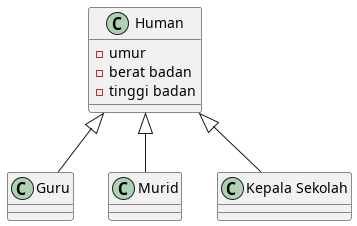
\includegraphics[width=8cm]{inheritance example.png}
              \caption{Contoh dari \textit{inheritance}}
          \end{figure}

    \item \textit{Polymorphism}

          \textit{Child class} adalah sebuah \textit{class} yang akan menuruni semua atribut dan fitur dari \textit{parent class}, tapi apabila dari satu \textit{parent class} memiliki 2 \textit{child class} yang memiliki fitur yang sama tapi cara melakukannya yang berbeda? contoh pisang goreng adalah sebuah makanan, tapi tidak semua makanan adalah pisang goreng, ada perubahan dari cara memasak dan cara penyajian ditiap - tiap makanan, disini konsep \textit{polymorphism} dapat dipakai. Secara definisi \textit{polymorphism} adalah kelakuan dimana \textit{child class} bisa melakukan suatu \textit{task} atau fitur yang sama seperti \textit{parent class} dengan cara yang berbeda\autocite{education-erin-oop-2020}.
\end{enumerate}


% \newpage
\subsubbab{2.1.2 \textit{Functional Programming}}
\textit{Functional Programming} adalah sebuah konsep, paradigma atau sebuah macam \textit{software development} yang menekankan titik beratnya pada penggunaan \textit{functions}, \textit{Functional Programming} sendiri bukan merupakan sebuah alat yang dapat digunakan tetapi merupakan sesuatu pegangan untuk \textit{developers} sebagai sebuah cara menulis kode\autocite{atencio2016functional}.


Tujuan dari \textit{Functional Programming} adalah membuat sebuah \textit{function} yang lebih kecil yang memiliki sifat dapat digunakkan kembali, lebih dapat diandalkan dan mudah dimengerti, lalu \textit{functions} tersebut maka akan dapat membuat sebuah program yang lebih dapat dimengerti \autocite{atencio2016functional}. \textit{Function} yang dibuat mengikuti \textit{Functional Programming} biasa dibuat dengan melakukan parameterisasi pada \textit{function} supaya dalam menggunakannya dengan menggunakkan parameter kode tersebut dapat digunakkan kembali untuk melakukan hal yang lain. \textit{Functional Programming} memiliki empat konsep dasar, yaitu \textit{Declarative programming}, \textit{Pure functions}, \textit{Referential transparency}, dan \textit{Immutability}\autocite{atencio2016functional}.


\begin{itemize}
    \item \textit{Declarative programming} adalah sebuah pendekatan \textit{programming} dimana sebuah kode untuk melakukan sesuatu akan ditulis menggunakan \textit{expressions} yang mendeskripsikan logika dari suatu program. Berbeda dengan Imperatif atau \textit{Procedural Programming} dimana akan ditulis secara detail bagaimana untuk melakukan sesuatu untuk mencapai hasil yang diinginkan\autocite{atencio2016functional}.
    \item \textit{Pure functions} adalah \textit{function} yang memiliki dua sifat, yaitu pertama, sebuah pure function hanya dan hanya bergantung pada input yang diberikan dan tidak dengan \textit{state} yang tersembunyi dan/atau external (diluar function tersebut) dan kedua, tidak merubah apapun yang diluar dari \textit{function} tersebut seperti obyek global atau parameter yang di \textit{pass} ke \textit{function} tersebut \autocite{atencio2016functional}.
    \item \textit{Referential transparency} adalah ketika sebuah \textit{function} menghasilkan hasil yang sama juga diberikan input yang sama \autocite{atencio2016functional}.
    \item \textit{Immutability} adalah dimana dalam \textit{Functional Programming} untuk melestarikan sebuah data supaya \textit{Immutable} tidak bisa diganti setelah di deklarasi. Dalam konsep ini yang perlu diperhatikan adalah object seperti \textit{array} yang dapat berubah konten atau valuenya dalam sebuah function \autocite{atencio2016functional}.
\end{itemize}

\subsubbab{2.1.3 \textit{Architectural Pattern}}
\textit{Architectural Pattern} merupakan seperangkat prinsip dan pola kasar yang menyediakan kerangka kerja abstrak dari sebuah sistem. \textit{Architectural Pattern} menggambarkan struktural fundamental dari suatu organisasi atau skema untuk sebuah sistem yang kompleks. \textit{Architectural Pattern} dapat digunakan sebagai solusi umum yang dapat digunakan kembali \textit{(reusable)} untuk memecahkan permasalahan yang biasa terjadi dalam sebuah \textit{software architecture} didalam konteks tertentu\autocite{architectural-pattern}. Dalam artian, \textit{Architectural Pattern} mirip dengan \textit{Design Pattern}, tetapi memiliki cakupan yang lebih luas\autocite{archi-pattern}.
\begin{itemize}
    \item \textit{Object-Oriented Architecture (OOA)}\\
          \textit{Object-Oriented Architecture} dapat digunakan jika ingin mengenkapsulasi logika dan data bersama-sama dalam komponen yang dapat digunakan kembali. \textit{Business Logic} yang kompleks yang membutuhkan abstraksi dan \textit{dynamic behaviour} dapat secara efektif menggunakan arsitektur jenis ini juga\autocite{architectural-pattern}.
    \item \textit{Layered/Tiered Architecture}\\
          \textit{Layered/Tiered Architecture} merupakan salah satu jenis \textit{architectural pattern} yang sangat sering digunakan\autocite{architectural-pattern}. Arsitektur jenis ini dapat digunakan untuk menyusun program yang dapat didekomposisikan menjadi beberapa kelompok \textit{subtasks}, yang masing-masing berada pada tingkat abstraksi tertentu. Setiap \textit{layer} menyediakan layanan \textit{(services)} ke \textit{layer} berikutnya yang lebih tinggi. Terdapat empat \textit{layer} utama didalam arsitektur jenis ini, yakni \textbf{\textit{Presentation Layer}}, \textbf{\textit{Application Layer}}, \textbf{\textit{Business Logic Layer}} dan \textbf{\textit{Data Access Layer}}. Arsitektur jenis ini biasanya digunakan pada aplikasi desktop dan \textit{web e-commerce} pada umumnya\autocite{archi-pattern}.
    \item \textit{Event-Driven Architecture (EDA)}\\
          \textit{Event-Driven Architecture (EDA)} biasanya didasarkan pada \textit{communication model} yang digerakkan oleh pesan asinkron untuk menyebarkan informasi ke seluruh organisasi/perusahaan. \textit{EDA} mendukung \textit{allignment} yang lebih alami dengan model operasional organisasi dengan menggambarkan \textit{business activity} nya sebagai suatu rangkaian \textit{event}/peristiwa\autocite{architectural-pattern}.
    \item \textit{Model-View-Controller Architecture (MVC)}\\
          \textit{Model-View-Controller Architecture} atau biasa juga disebut sebagai \textbf{MVC}, merupakan sebuah jenis \textit{architectural pattern} yang membagi sistem aplikasinya menjadi tiga bagian, yakni \textbf{\textit{Model}}, \textbf{\textit{View}} dan \textbf{\textit{Controller}}. \textbf{\textit{Model}} merupakan fungsi inti dari aplikasi dan menyimpan data, \textbf{\textit{View}} merupakan sebuah \textit{user interface (UI)} yang dapat dilihat atau berinteraksi dengan pengguna secara langsung dan \textbf{\textit{Controller}} sebagai penghubung antara \textit{model} dengan \textit{view} serta yang mengatur \textit{input} dari pengguna. Arsitektur jenis ini paling sering digunakan untuk membuat sebuah aplikasi berbasis \textit{web}\autocite{archi-pattern}.
\end{itemize}

\subsubbab{2.1.4 \textit{Design Pattern}}
\textit{Design Pattern} secara definisi adalah sesuatu cara komunikasi tiap obyek dan \textit{class} yang dikostumisasi untuk memecahkan masalah desain general didalam konteks tertentu, \textit{design pattern} membantu untuk membuat \textit{object oriented design} yang dapat digunakan secara berulang, dengan cara memberi nama, mengabstraksi, dna mengidentifikasi kunci aspek dari struktur desain tertentu\autocite{design-pattern-2588942}.
\begin{itemize}
    \item \textit{Facade}\\
          \textit{Facade} adalah sesuatu \textit{class} yang memberikan \textit{interface} yang simpel ke sub-sistem yang kompleks, \textit{design pattern} ini dapat digunakan ketika butuh mengintegrasikan sesuatu \textit{library} dengan fitur yang sangat banyak tapi hanya butuh menggunakan beberapa fiturnya saja\autocite{refactoring-guru}. \textit{Singleton} juga memberikan global \textit{access point} ke instansi \textit{class} tersebut, jadi semua \textit{class} dan \textit{object} dapat membaca \textit{value} yang sama dan merubah \textit{value} tersebut secara keseluruhan\autocite{refactoring-guru}.
    \item \textit{Singleton}\\
          \textit{Singleton} digunakan untuk menjamin bahwa suatu \textit{class} hanya memiliki satu \textit{instance}, \textit{design pattern} ini berguna saat ingin mengontrol sebuah \textit{shared resources} seperti \textit{database}\autocite{refactoring-guru}.
    \item \textit{Builder}\\
          \textit{Design pattern} ini dibuat untuk memecahkan masalah ketika ada sebuah \textit{class} yang saat dibuat menjadi sebuah \textit{object} tidak semua atributnya diisi, tanpa harus membuat \textit{contructor} atau \textit{child class} banyak. \textit{Builder} mengekstrasi \textit{building steps} saat membuat suatu \textit{object} dari sebuah \textit{class} dan memindahkannya ke \textit{class} terpisah\autocite{refactoring-guru}.
    \item \textit{Template Method}\\
          \textit{Template method} digunakan untuk mengurangi redudansi ketika ada beberapa fitur dengan langkah penyelesaian sama tapi dengan cara yang berbeda, \textit{template method} dibuat dengan cara memisahkan logika suatu fitur menjadi beberapa langkah dan saat ingin menambahkan fitur baru, bisa langsung membuat \textit{child class} dari \textit{template method} tersebut dan meng-\textit{override} step yang ingin diganti logikanya\autocite{refactoring-guru}.
\end{itemize}

\subsubbab{2.1.5 \textit{Software Testing}}

Secara general manusia pasti akan melakukan kesalahan, apa lagi didalam \textit{software development} hal ini sangat kelihatan saat dengan pasti adanya \textit{bug} didalam \textit{software} yang dikerjakan, ini adalah salah satu alasan kenapa \textit{software testing} itu dibutuhkan, untuk menemukan masalah dan memperbaikinya. Alasan satu lagi \textit{software testing} dilakukan adalah untuk membuat keputusan, apakah \textit{software} yang sedang dibuat ini sudah mempunyai kualitas yang dapat diterima \autocite{jorgensen2018software}.

Secara definisi dasar, \textit{software testing} adalah suatu metode untuk mengecek apakah sebuah produk atau \textit{software} sudah sama dengan kebutuhan - kebutuhan dan memastikan \textit{software} tersebut tidak memiliki kecacatan\autocite{guru99-software-testing}.

\textit{Software testing} bisa digeneralisasikan menjadi 2 tipe, yaitu:
\begin{itemize}
    \item \textit{Blackbox testing}

        \textit{Blackbox testing} atau sering disebut \textit{specification-based testing}, adalah testing yang dilakukan bedasarkan dengan spesifikasi \textit{software} tersebut. Metode testing ini disebut \textit{blackbox testing} karena sebuah sistem atau program itu akan dianggap seperti kotak hitam yang tidak bisa dilihat isinya, tapi diketahui apa saja yang bisa dilakukan oleh kotak hitam tersebut\autocite{jorgensen2018software}.

        Kelebihan dari metode \textit{testing} ini adalah, \textit{unit test} yang dibuat itu berdiri sendiri dari bagaimana impelmentasi yang ada didalam \textit{software} tersebut, jadi jika ada perubahan implementasi \textit{test case} yang sebelumnya dibuat akan tetap bisa dipakai dan \textit{testcase} untuk \textit{blackbox testing} dapat dibuat saat masa \textit{development} sedang berjalan, jadi bisa mengurangi masa pengerjaan \textit{project}\autocite{jorgensen2018software}.


    \item \textit{Whitebox testing}

        \textit{Whitebox testing} adalah metode \textit{testing} yang dimana semua struktur internal, desain, dan implementasi dites untuk memperbaiki desain, kegunaan, dan keamanan. Terminologi \textit{whitebox} ini menganggap \textit{software} itu seperti box yang transparan, dimana semua isinya (implementasi dari sebuah fungsi dan pilihan desain yang diambil) akan kelihatan dalam fase pengetesan\autocite{guru99-whitebox-testing}.

        Salah satu tipe \textit{whitebox testing} adalah \textit{unit testing}. \textit{Unit testing} adalah \textit{test case} yang biasanya ditulis oleh \textit{developer} untuk melakukan pengetesan disetiap blok kode yang sedang dikembangkan\autocite{guru99-whitebox-testing}. Ada dua teknik yang bisa diterapkan saat melakukan \textit{whitebox testing}, yaitu:
        \begin{itemize}
            \item \textit{Statement Coverage}

            teknik ini membutuhkan semua \textit{statement} yang ada didalam \textit{code base} sudah tertutupi oleh \textit{test case} dari \textit{whitebox testing}.
 
            \item \textit{Branch Coverage}

            teknik ini membutuhkan semua \textit{branch} atau \textit{path} yang ada didalam \textit{code base} sudah tertutupi oleh \textit{test case} dari \textit{whitebox testing}.
        \end{itemize}
\end{itemize}

\subsubbab{2.1.6 Sistem Rekomendasi}
Sistem rekomendasi adalah sistem penyaringan informasi yang menyarankan sebuah produk kepada pengguna bedasarkan preferensi atau perilaku masa lalu. Sistem ini banyak digunakan di pasar \textit{online} untuk meningkatkan pengalaman, keterlibatan pengguna, dan mendorong penjualan. Dengan memberikan rekomendasi yang dipersonalisasi terhadap preferensi, pengguna dapat menemukan sebuah barang yang mungkin tidak bisa ditemukan sendiri dan meningkatkan kepuasan pengguna terhadap pasar \textit{online} yang sedang digunakan \autocite{adiwardana2019}.

Kenapa sistem rekomendasi ini dibutuhkan telah dibuktikan oleh sebuah artikel yang diterbitkan pada tahun 2019 oleh Tian \textit{et al}. yang berjudul "\textit{Exploring the effects of personalized recommendation on users' satisfaction and loyalty in e-commerce}" yang menemukan bahwa pengguna \textit{platform e-commerce}  akan menghabiskan waktu 50\% lebih banyak di \textit{platform} tersebut ketika pengguna diberikan sebuah rekomendasi produk yang dipersonalisasi\autocite{tian2019exploring}. Sistem rekomendasi juga menguntungkan untuk mengurangi terjadinya \textit{information overload} yang akan dialami oleh pengguna, dengan cara hanya menampilkan produk yang ingin dilihat atau yang sesuai dengan preferensi - preferensi pengguna tersebut\autocite{karimi2018news}.

Sistem rekomendasi yang akan dipakai didalam proyek ini akan berdasarkan pada teori \textit{Knowledge Graph}. \textit{Knowledge Graph} adalah sebuah \textit{graph} heterogen, dimana \textit{nodes} akan merepresentasikan sebuah hubungan antara entitas\autocite{guo2020survey}. Dengan menggunakan teori ini, semua produk dan atribut - atributnya dapat dibuat menjadi sebuah \textit{graph} untuk mempermudah memahami hubungan antara tiap produk, selain itu informasi pengguna dan preferensi mereka-pun bisa diintegrasikan ke-\textit{graph} tersebut untuk membantu prediksi rekomendasi menjadi seakurat mungkin.

\begin{figure}[h]
    \centering
    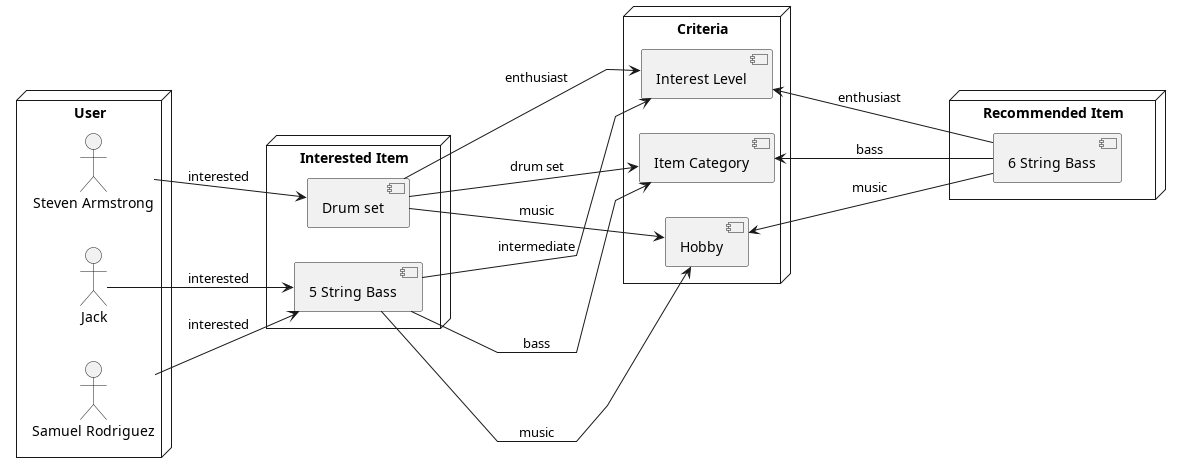
\includegraphics[width=8cm]{recommendation system architecture.png}
    \caption{Contoh simpel dari sistem rekomendasi dengan basis \textit{Knowledge Graph}}
\end{figure}

\subsubbab{2.1.7 \textit{Caching}}
Secara definisi \textit{caching} adalah sebuah \textit{data storage layer} yang bersifat sementara dan digunakan untuk mempercepat permintaan data dibanding mekases lokasi penyimpanan utama data tersebut. Fungsi utama \textit{cache} adalah menurunkan proses permintaan data ke lokasi penyimpanan utama yang lambat dengan cara menaruh data tersebut ke \textit{storage layer} yang lebih cepat seperti RAM\autocite{AWS-caching}. Berikut adalah kelebihan dari sistem \textit{caching}:

\begin{itemize}
    \item \textit{Cache} membuat semuanya berjalan lebih cepat. Manfaat utama dari cache adalah menurunkan \textit{response time} yang dibutuhkan untuk memproses sebuah \textit{request}. Seperti contoh, dengan menyimpan salinan lokan file dari sebuah \textit{website} saat pertama kali dikunjungi, pada kunjungan berikutnya browser tidak perlu membuang waktu dan sumber daya untuk mengunduh informasi tersebut karena sudah disimpan di penyimpanan lokal\autocite{businessinsider_cache}.

    \item Menghilangi \textit{Database Hotspot}. Dibanyak aplikasi kemungkinan hanya sebagian kecil data yang akan diakses lebih sering dibandingkan dengan data lainnya, seperti profile selebriti yang terkenal atau produk yang diminati banyak orang. Hal ini dapat menyebabkan \textit{hot spots} di \textit{database} yang digunakan dan mungkin memerlukan penyediaan \textit{resource database} yang berlebihan bedasarkan \textit{throughput} atau jumlah data yang dapat ditangani\autocite{AWS-caching}. \textit{Cache} mengatasi hal ini dengan memunkinkan \textit{software} untuk mengakses memori lokalnya seperti RAM dibandingkan membuat \textit{request} untuk meng-\textit{query} data dari \textit{database}, yang dapat menjadi operasi yang mahal.

    \item \textit{Cache} juga bisa mengurangi beban di \textit{backend}, dengan cara mengalihkan sebagian besar beban operasi \textit{query} ke memori lokal dari \textit{database backend}, hal ini akan mencegah terjadinya performa yang menurun atau \textit{crashing} ketika ada lonjakan \textit{traffic}.
\end{itemize}



\subsubbab{2.1.8 \textit{Asynchronous Processing}}

\subbab{2.2 Aplikasi Serupa}
Berikut adalah perbandingan antara beberapa aplikasi serupa dari hasil penelitian-penelitian terdahulu dan dua aplikasi pasaran yang sebelumnya sudah sedikit dibahas pada bagian latar belakang. Disini, aplikasi-aplikasi tersebut dapat dikategorikan menjadi dua jenis, yaitu \textit{marketplace} atau \textit{e-commerce} dan sebuah forum untuk berdiskusi secara general. Berikut adalah perbandingan kelebihan dan kekurangannya.
\textbf{Aplikasi-aplikasi berdasarkan penelitian terdahulu}:
\begin{longtable}{|p{3cm}|p{5cm}|p{5cm}|}
    \hline
    Aplikasi & Positif                                                                                                                 & Negatif \\
    \hline
    Application for Marketplace Agricultural Product
             & + Mempermudah para petani/pekebun untuk menjual belikan produk agrikulturnya \newline
    + User dapat me-\textit{request} produk yang belum ada agar bisa dijual di app tersebut \newline
             & - Hanya terfokus terhadap satu sektor saja yaitu agrikultur \newline
    - Tidak bisa berdiskusi langsung dengan penjual mengenai produk yg dijual \newline
    - Bukan \textit{marketplace} untuk hobi \newline
    - Hanya tersedia di satu kota saja \newline
    - Hanya bisa berjalan di Android saja, tidak bisa di IOS                                                                                     \\
    \hline
    e-Nelayan the Fishery Marketplace App
             & + Mempermudah para nelayan dan penjual ikan untuk menjual belikan ikan-ikannya \newline
    + User dapat me-\textit{request} ikan yang belum tersedia dengan membuat post agar bisa dilihat langsung oleh nelayan atau penjual ikan \newline
    + App ini dapat menghubungankan pihak user, penjual hingga nelayan melalui sistem comment pada postingan user \newline
             & - Hanya terfokus pada sektor perikanan saja \newline
    - Bukan \textit{marketplace} untuk hobi \newline
    - Hanya bisa berjalan di Android saja, tidak bisa di IOS                                                                                     \\
    \hline
    LIDI: A Web-Based Car Rent Marketplace Application
             & + Mempermudah user yang ingin menyewa mobil secara online \newline
    + Menampilkan informasi lengkap mengenai mobil yang disewakan \newline
             & - Hanya terfokus pada jasa sewa mobil \newline
    - Proses \textit{order} masih menggunakan antrian \textit{via} nomor telepon user \newline
    - User harus secara manual mengecek sendiri kondisi mobil yang ingin disewa \newline
    - Hanya tersedia di satu kota saja \newline
    - Bukan \textit{marketplace} khusus untuk hobi                                                                                               \\
    \hline
    e-Marketplace for Village-owned Small, Micro and Medium Enterprise
             & + Mempermudah user untuk mencari produk yang hanya dijual oleh bisnis-bisnis kecil \newline
    + Memepersatukan bisnis-bisnis kecil kedalam satu \textit{platform} online jual beli yang sama \newline
             & - \textit{User Interface} yang masih minim penjelasannya yang dapat membuat user kebingungan \newline
    - Hanya tersedia di satu lokasi saja \newline
    - Bukan \textit{marketplace} khusus untuk hobi                                                                                               \\
    \hline
    C2C marketplace model in fishery product trading application
             & + User dan nelayan dapat dengan mudah berinteraksi walaupun berada di pedesaan dengan infrastruktur yang jelek \newline
    + Sistem yang relatif simpel \newline
             & - Hanya terfokus pada sektor perikanan saja \newline
    - Hanya tersedia di satu lokasi saja \newline
    - Bukan \textit{marketplace} khusus untuk keperluan hobi                                                                                     \\
    \hline
\end{longtable}

\textbf{Aplikasi pasaran yang serupa dengan proyek ini}:
\begin{longtable}{|m{3cm}|p{5cm}|p{5cm}|}
    \hline
    Aplikasi & Positif                                                  & Negatif                \\
    \hline
    KyouId
             & + Bisa membeli barang dari negara lain (Jepang) \newline
    + Sudah integrasi langsung dengan banyak \textit{shipment service} yang ada di Indonesia \newline
             & - Hanya terfokus kesatu jenis hobi \newline
    - Tidak memiliki filter untuk \textit{interest level}                                        \\
    \hline
    Reddit
             & + \textit{community} yang sudah besar \newline
    + System handling \textit{post} dan komen sudah \textit{robust} \newline
    + Interaksi antara user sudah bagus
             & - Bukan marketplace \newline
    - Tidak cocok untuk memberi rating konkrit kepada barang \newline
    - Tidak ada gambar atau suatu panel untuk menampilkan informasi item tersebut secara singkat \\
    \hline
\end{longtable}


\newpage
\bab{Bab 3. Metode Penelitian}
\subbab{3.1 Metode Penelitian}

Pengumpulan data yang lakukan adalah dengan membuat form survei menggunakan \textit{Google Form} untuk mendapatkan pendapat atas pertanyaan-pertanyaan yang terkait dengan alasan dari pembuatan aplikasi pada proyek ini. Dari hal mengenai pembelian barang hobi hingga tingkat kesulitan dalam menemukan barang yang cocok. Dari semua jawaban survei yang dikumpulkan tersebutlah, dapat memperoleh gambaran dan konfirmasi atas fitur-fitur yang proyek ini butuhkan.


Pertanyaan “Apakah anda takut untuk mengambil hobi baru karena tidak tau mulai dari mana?”, diajukan kepada pengisi survei untuk mendapatkan data dan konfirmasi apakah aplikasi dalam proyek ini dibutuhkan, dan dengan hasil jawaban mayoritas diatas 60\% menjawab iya, dari data tersebut bisa disimpulkan adanya kesulitan memulai hobi karena keraguan titik mulai hobi tersebut.


Selanjutnya dengan “Apakah anda sering menggunakan \textit{e-commerce} untuk browsing dan mencari barang berhubungan dengan hobi anda?” untuk validasi apakah menggunakkan fasilitas online untuk membeli barang hobi itu merupakan metode yang populer. Dengan masukan yang didapatkan dari survei, 70\% menjawab iya maka dapat disimpulkan bahwa fasilitas jual/beli barang hobi di internet itu layak dilakukan.


Pertanyaan “Dalam mencari dan menemukan barang apakah anda terkadang merasa ragu dan harus mencari tahu terlebih dahulu atas barang yang anda lihat apakah untuk pemula/menengah/ahli?” ini adalah untuk mengumpulkan data atas fitur utama yang dirancang yaitu fitur filtrasi level peminatan(\textit{interest level}) dari suatu hobi Dengan respons yang berjawab iya diatas 70\% maka fitur utama dari proyek ini layak untuk diimplementasikan.

\subbab{3.2 Metode Pengembangan Sistem}

\subsubbab{3.2.1 \textit{Software Design Document}}
\begin{enumerate}[label=\alph*. ]
    \item Deskripsi \textit{software}

          \textit{Shumishumi} adalah sebuah marketplace dimana user bisa membeli suatu barang sesuai dengan hobi dan setinggi apa \textit{interest level} mereka. Tujuan dari aplikasi ini adalah mempermudah pengguna pembeli untuk mencari barang hobi yang cocok, mempermudah penjual dalam mempromosikan barang-nya kepada pelanggan dengan fitur filter \textit{Interest Level}.


          \textit{Shumishumi} juga bisa menjadi sarana untuk berdiskusi mengenai topik dan hobi yang diminati, dengan fitur ini \textit{user} diharapkan dapat mencari hobi baru dengan mudah.

    \item Fungsi-fungsi \textit{software}


          Fungsi dari proyek ini dibagi menjadi dua perspektif, perspektif dari pembeli dan perspektif dari penjual.
          \begin{itemize}
              \item Perspektif dari pembeli

                    Pembeli bisa mencari sebuah barang secara spesifik menggunakan nama atau siapa yang menjual barang tersebut, tapi bagi penjual yang baru ingin memasuki suatu hobi, mereka bisa mengutilisasikan fitur filter bedasarkan hobi apa yang ingin mereka masuki dan \textit{interest level} mereka. Selain itu juga pembeli juga bisa membuat review tentang barang yang mereka jual, bagaimana kualitas dari barang tersebut dan apakah barang tersebut memenuhi kriteria \textit{interest level} yang ditujukkan.

                    Selain itu juga pembeli bisa membuat suatu \textit{post} atau \textit{comment} tentang hobi mereka, atau membaca \textit{post} yang sudah dibuat oleh pembeli lain untuk membantu mereka mendalami hobi yang mereka punya.

              \item Perspektif dari penjual

                    Penjual bisa menjual barang, saat memasukan barang yang ingin dijual penjual harus memasukan barang itu terkait dengan hobi apa dan ditujukkan ke \textit{interest level} mana, selain itu penjual juga bisa melihat sebuah \textit{dashboard} yang berisikan \textit{review} dari pembeli dan berapa banyak barang yang sudah mereka jual.
          \end{itemize}

          % sequence diagram

    \item Kebutuhan teknologi

          \begin{enumerate}
              \item \textit{Software Development Life-Cycle - Agile}\\
                    \textbf{SDLC} yang dipakai dalam proyek ini adalah \textit{Agile}, dikarenakan \textit{agile} dapat membantu proyek ini dikerjakan dalam \textit{size} yang lebih kecil dan bisa diwujudkan dengan \textit{timeframe} yang masuk akal dan bersifat \textit{continuous} jadi lebih fleksible saat menghadapi perubahan \textit{requirement}\autocite{atlassian-agile}.

              \item \textit{Back end}

                    \textit{Back end} atau bisa disebut juga \textit{developer's end} adalah sebuah layer yang memproses semuanya dibelakang layar dan tempat terjadinya sesuatu yang tidak bisa dilihat oleh \textit{user}\autocite{letsgodojo-frontend-backend}. Analogy yang bisa digunakan adalah saat disebuah restoran ada pelanggan yang memesan sesuatu yang spesifik ke pelayan, ini adalah bagian \textit{front end} dari restoran tersebut, setelah itu pelayan memberikan pesanan tersebut ke koki, yang akan mengambil bahan masak, momotong semua bahan - bahan tersebut, dan memasaknya sesuai resep yang sudah dibuat, koki ini yang merepresentasikan bagian \textit{backend} dari restoran tersebut\autocite{codecademy-backend}.

                    \textit{Back end} terdiri dari dua hal, \textit{servers} yang akan meproses data dan \textit{request} dari sebuah user dan \textit{database} yang akan menyimpan data yang sudah atau yang akan mau diproses\autocite{codecademy-backend}. Proyek ini akan menggunakan \textit{springboot} sebagai \textit{framework} yang digunakan untuk membuat \textit{software back end}-nya dan \textit{\textbf{MySQL}} sebagai database yang digunakan.

                    \textit{Springboot} adalah \textit{java back end framework} yang paling populer didunia, \textit{springboot} membuat menulis \textit{software back end} menjadi lebih mudah dan lebih cepat\autocite{spring-framework}, alasan kenapa proyek ini menggunakan \textit{springboot} adalah sebagai berikut:
                    \begin{itemize}
                        \item \textit{Springboot} mempunyai banyak \textit{plugin} yang dapat di\textit{install};
                        \item komunitas \textit{springboot} itu sangat besar;
                        \item dan yang terakhir \textit{springboot} memiliki fitur \textit{Inversion of Control} dan \textit{Dependency Injection}.
                    \end{itemize}

              \item \textit{Front end}

                    \textit{Front End} adalah sebuah bagian dari halaman web yang dimana merupakan tempat interaksi pengguna, \textit{Front End} sebagai tempat interaksi pengguna maka merupakan bagian dari sebuah halaman yang sangat sering dilihat oleh pengguna kebalikan dari \textit{Back End}\autocite{codecademy-frontend}.

                    \textit{Javascript} adalah bahasa pemrograman terkompilasi yang memiliki karakteristik ringan untuk dijalankan, \textit{interpreted} dan juga dengan fitur \textit{first-class functions} dimana \textit{function} dianggap seperti variabel biasa lainnya seperti \textit{string, number,} dan lain-lain. Yang dimana penggunaan \textit{Javascript} paling terkenal dan banyak digunakkan adalah dalam bahasa untuk \textit{Web} atau situs internet\autocite{javascript-mdn}.

                    \textit{Typescript} adalah bahasa pemrograman yang dibuat untuk memecahkan beberapa permasalahan yang ada di dalam bahasa \textit{Javascript}, salah satu contohnya adalah dengan \textit{Typescript} penggunaan \textit{Type-annotation} dapat digunakkan untuk memberi tipe dari variabel sehingga permasalahan yang mungkin dapat muncul karena karakteristik \textit{Javascript} yang \textit{loosely typed} dapat diatasi\autocite{fenton2014pro}.

                    \textit{React} adalah sebuah Library untuk bahasa pemrograman \textit{Javascript} (\textit{Typescript} juga bisa) untuk membuat \textit{UI}. Fitur dari \textit{React} adalah \textit{React} menganut \textit{Declarative Programming} dan juga \textit{Functional Programming},\textit{Component Based}, \textit{Hooks} dan \textit{Lifecycle Hooks}\autocite{react-general}. \textit{Hooks} dan \textit{Lifecycle Hooks} adalah sebuah fitur yang diimplementasikan pada \textit{React v16.8} yang memberi alternatif dari menggunakkan \textit{class} untuk komponen\autocite{react-hooks, react-hooks-lifecycle}.

          \end{enumerate}

\end{enumerate}


\newpage
\subsubbab{3.2.2 Perancangan Sistem}
% \subsubsection*{3.2.2 \textit{Timeline}}
% \addcontentsline{toc}{subsubsection}{\protect\numberline{}3.2.2 \textit{Timeline}}

% Karena proyek ini menggunakan \textit{agile} sebagai \textbf{SDLC} yang digunakan, maka \textit{timeline} ini dipisah menjadi satu bulan pertama untuk \textit{planning} dan lima bulan yangd dipisah menjadi lima \textit{sprint} yang berbeda. Dalam satu \textit{sprint} akan dipisah lagi menjadi satu minggu pertama untuk melakukan \textit{spring planning}, dua minggu untuk masa \textit{development frontend} dan \textit{backend} secara bersamaan dan satu minggu akan dipakai untuk masa \textit{testing} untuk memastikan fitur yang di\textit{develop} tidak menggangu fitur yang sudah ada dan bisa digunakan.

% \begin{figure}[h]
%     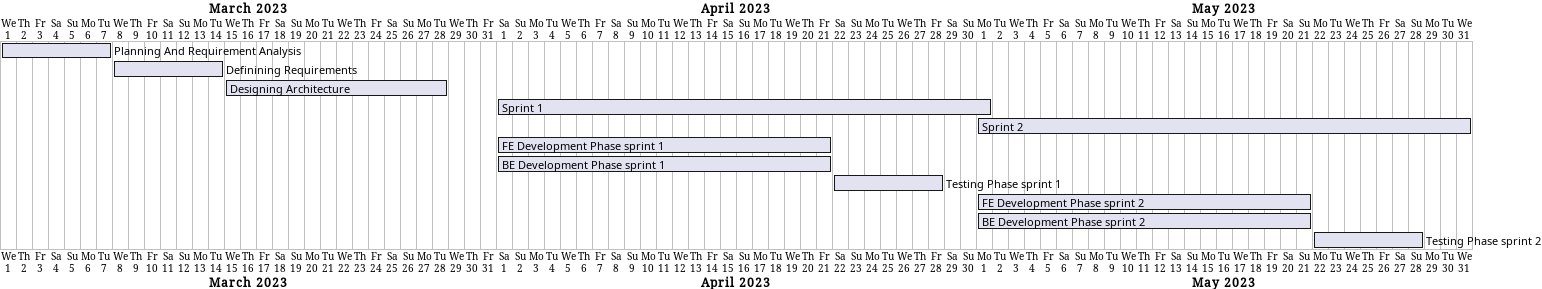
\includegraphics[width=13cm]{sprint timeline.png}
%     \centering
%     \caption{\textit{Timeline} untuk bulan maret sampai mei.}
% \end{figure}

% \begin{figure}[h]
%     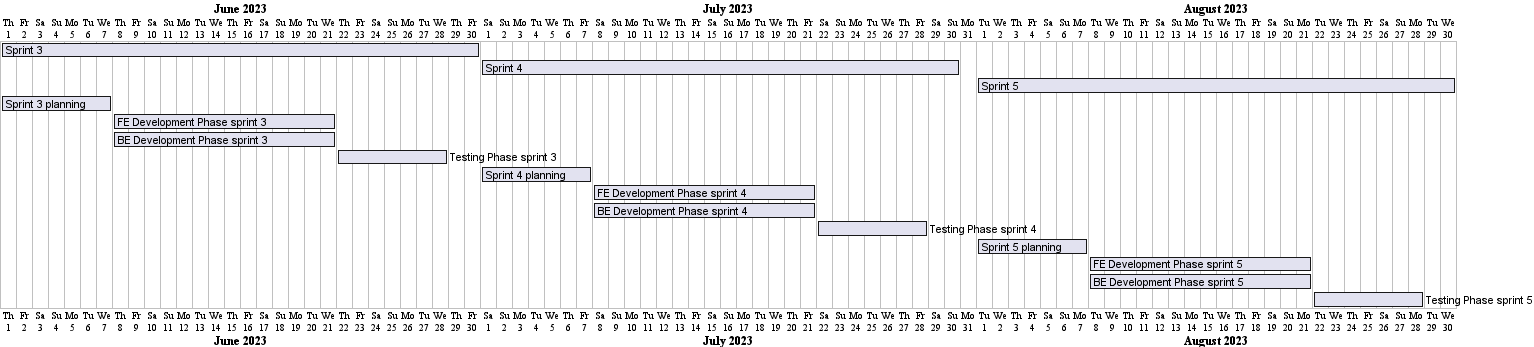
\includegraphics[width=13cm]{sprint timeline 2.png}
%     \centering
%     \caption{\textit{Timeline} untuk bulan juni sampai agustus.}
% \end{figure}

\newpage


% \subsubsection*{3.2.2 Perancangan Sistem}
% \addcontentsline{toc}{subsubsection}{\protect\numberline{}3.2.2 Perancangan Sistem}
% \begin{enumerate}
%     \item Desain \textit{database}\\
%     \begin{figure}[h]
%         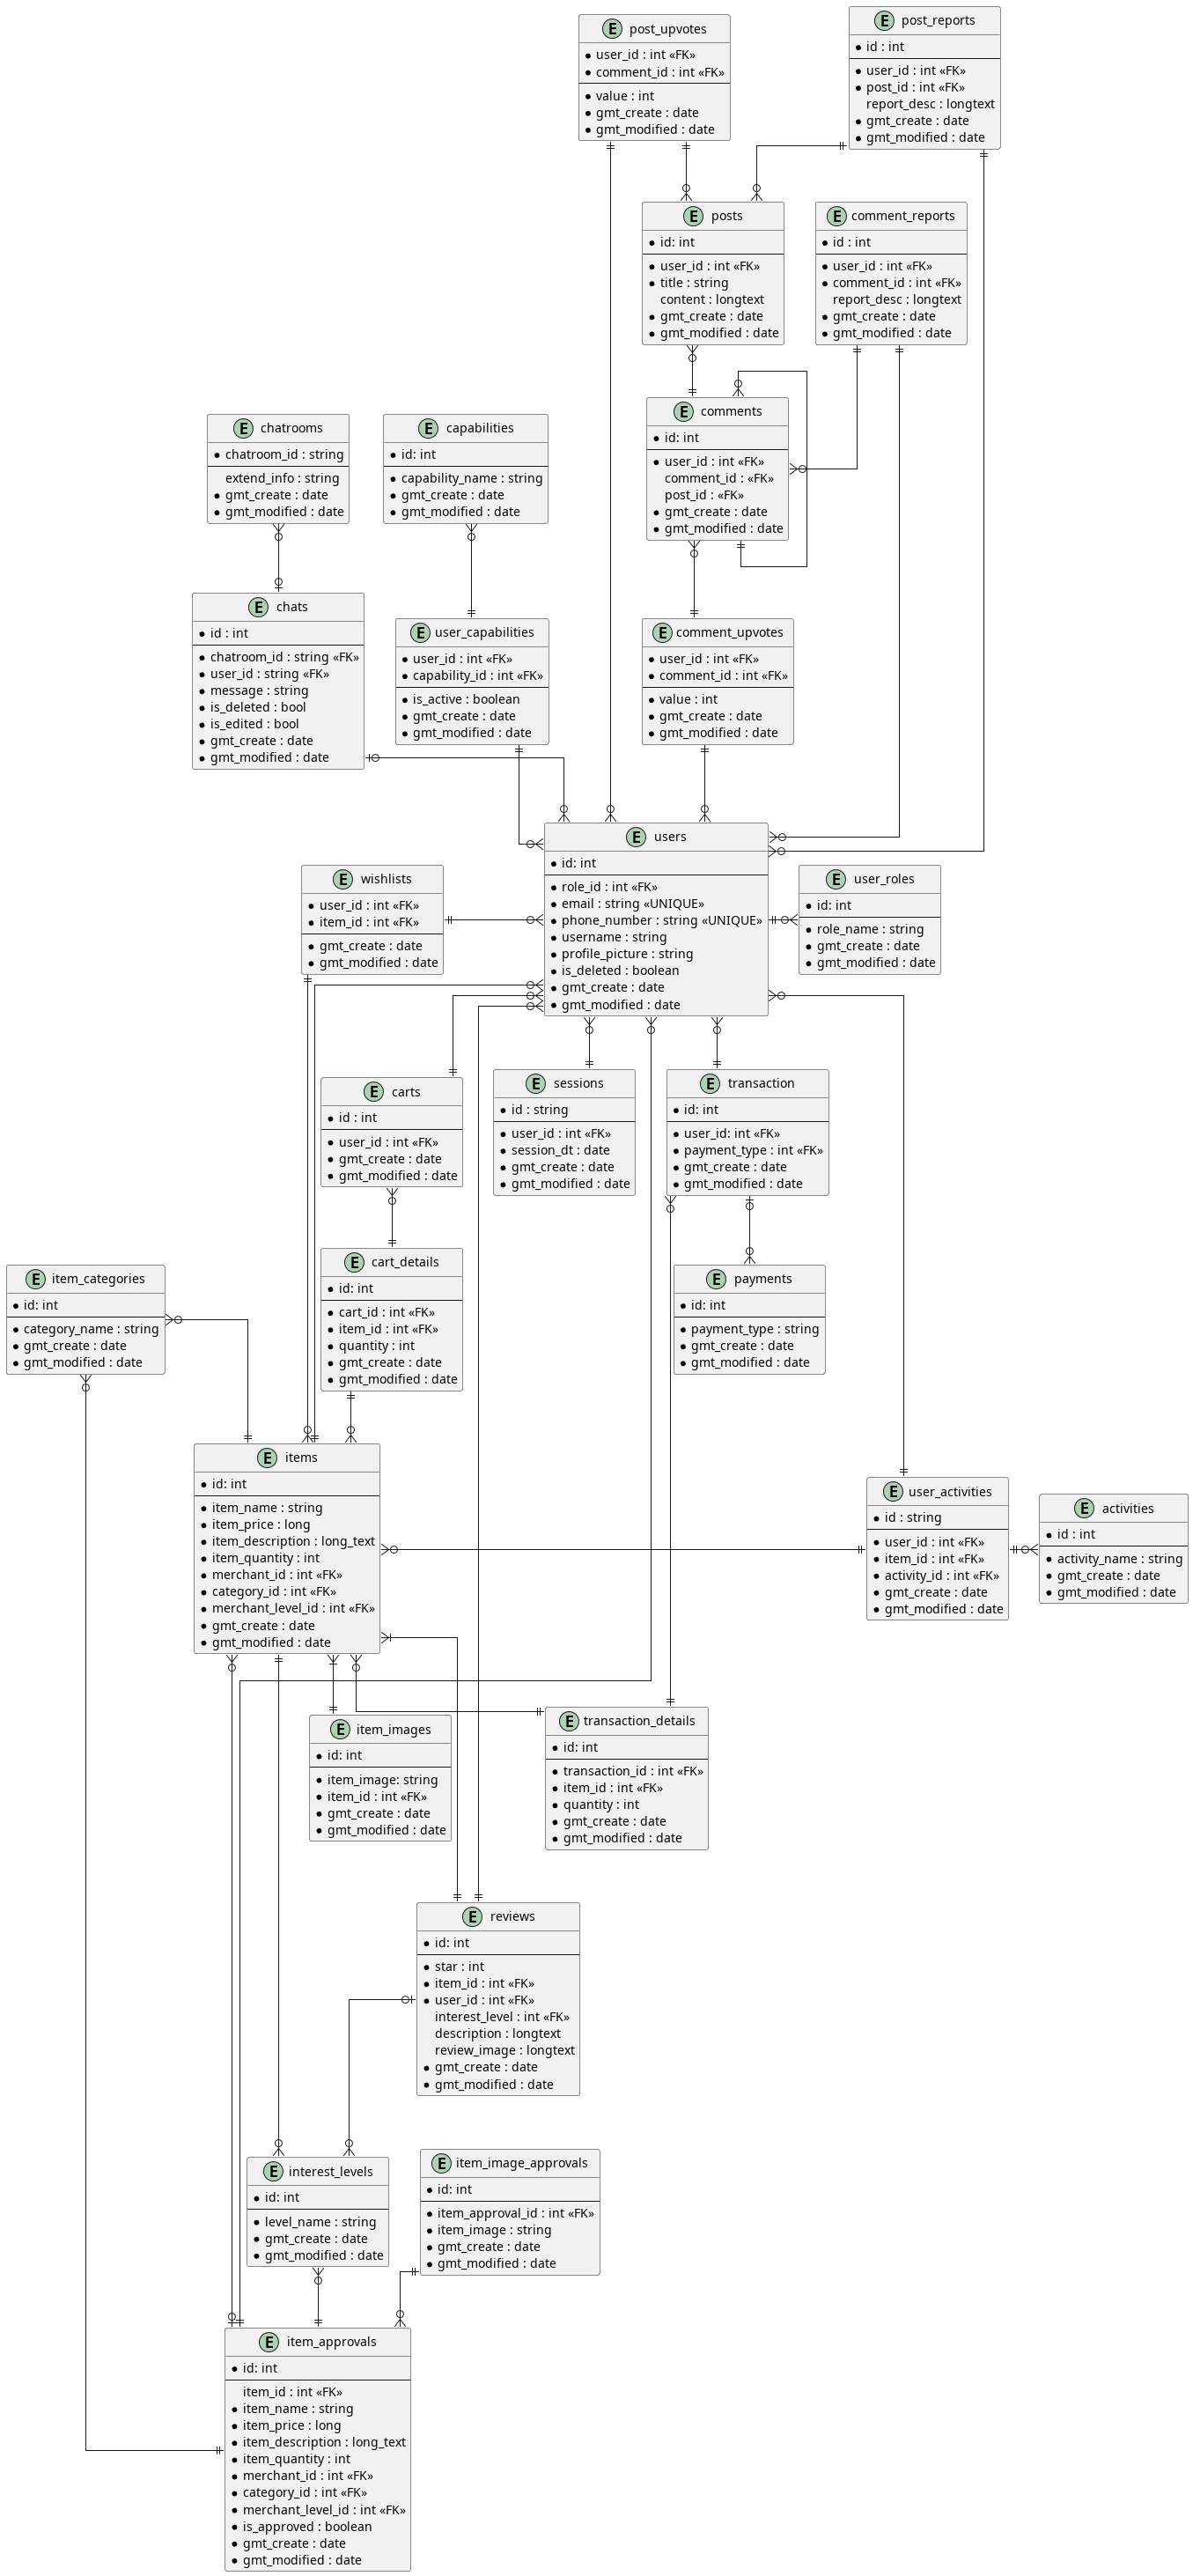
\includegraphics[height=12cm,keepaspectratio]{erd diagram.png}
%         \centering
%         \caption{\textit{Entity Relation Diagram}}
%     \end{figure}
%     \newpage
%     \item \textit{Sequence Diagram}\\
%     \begin{itemize}
%         \item \textit{Buyer flow sequence diagram}\\
%             \begin{figure}[h]
%                 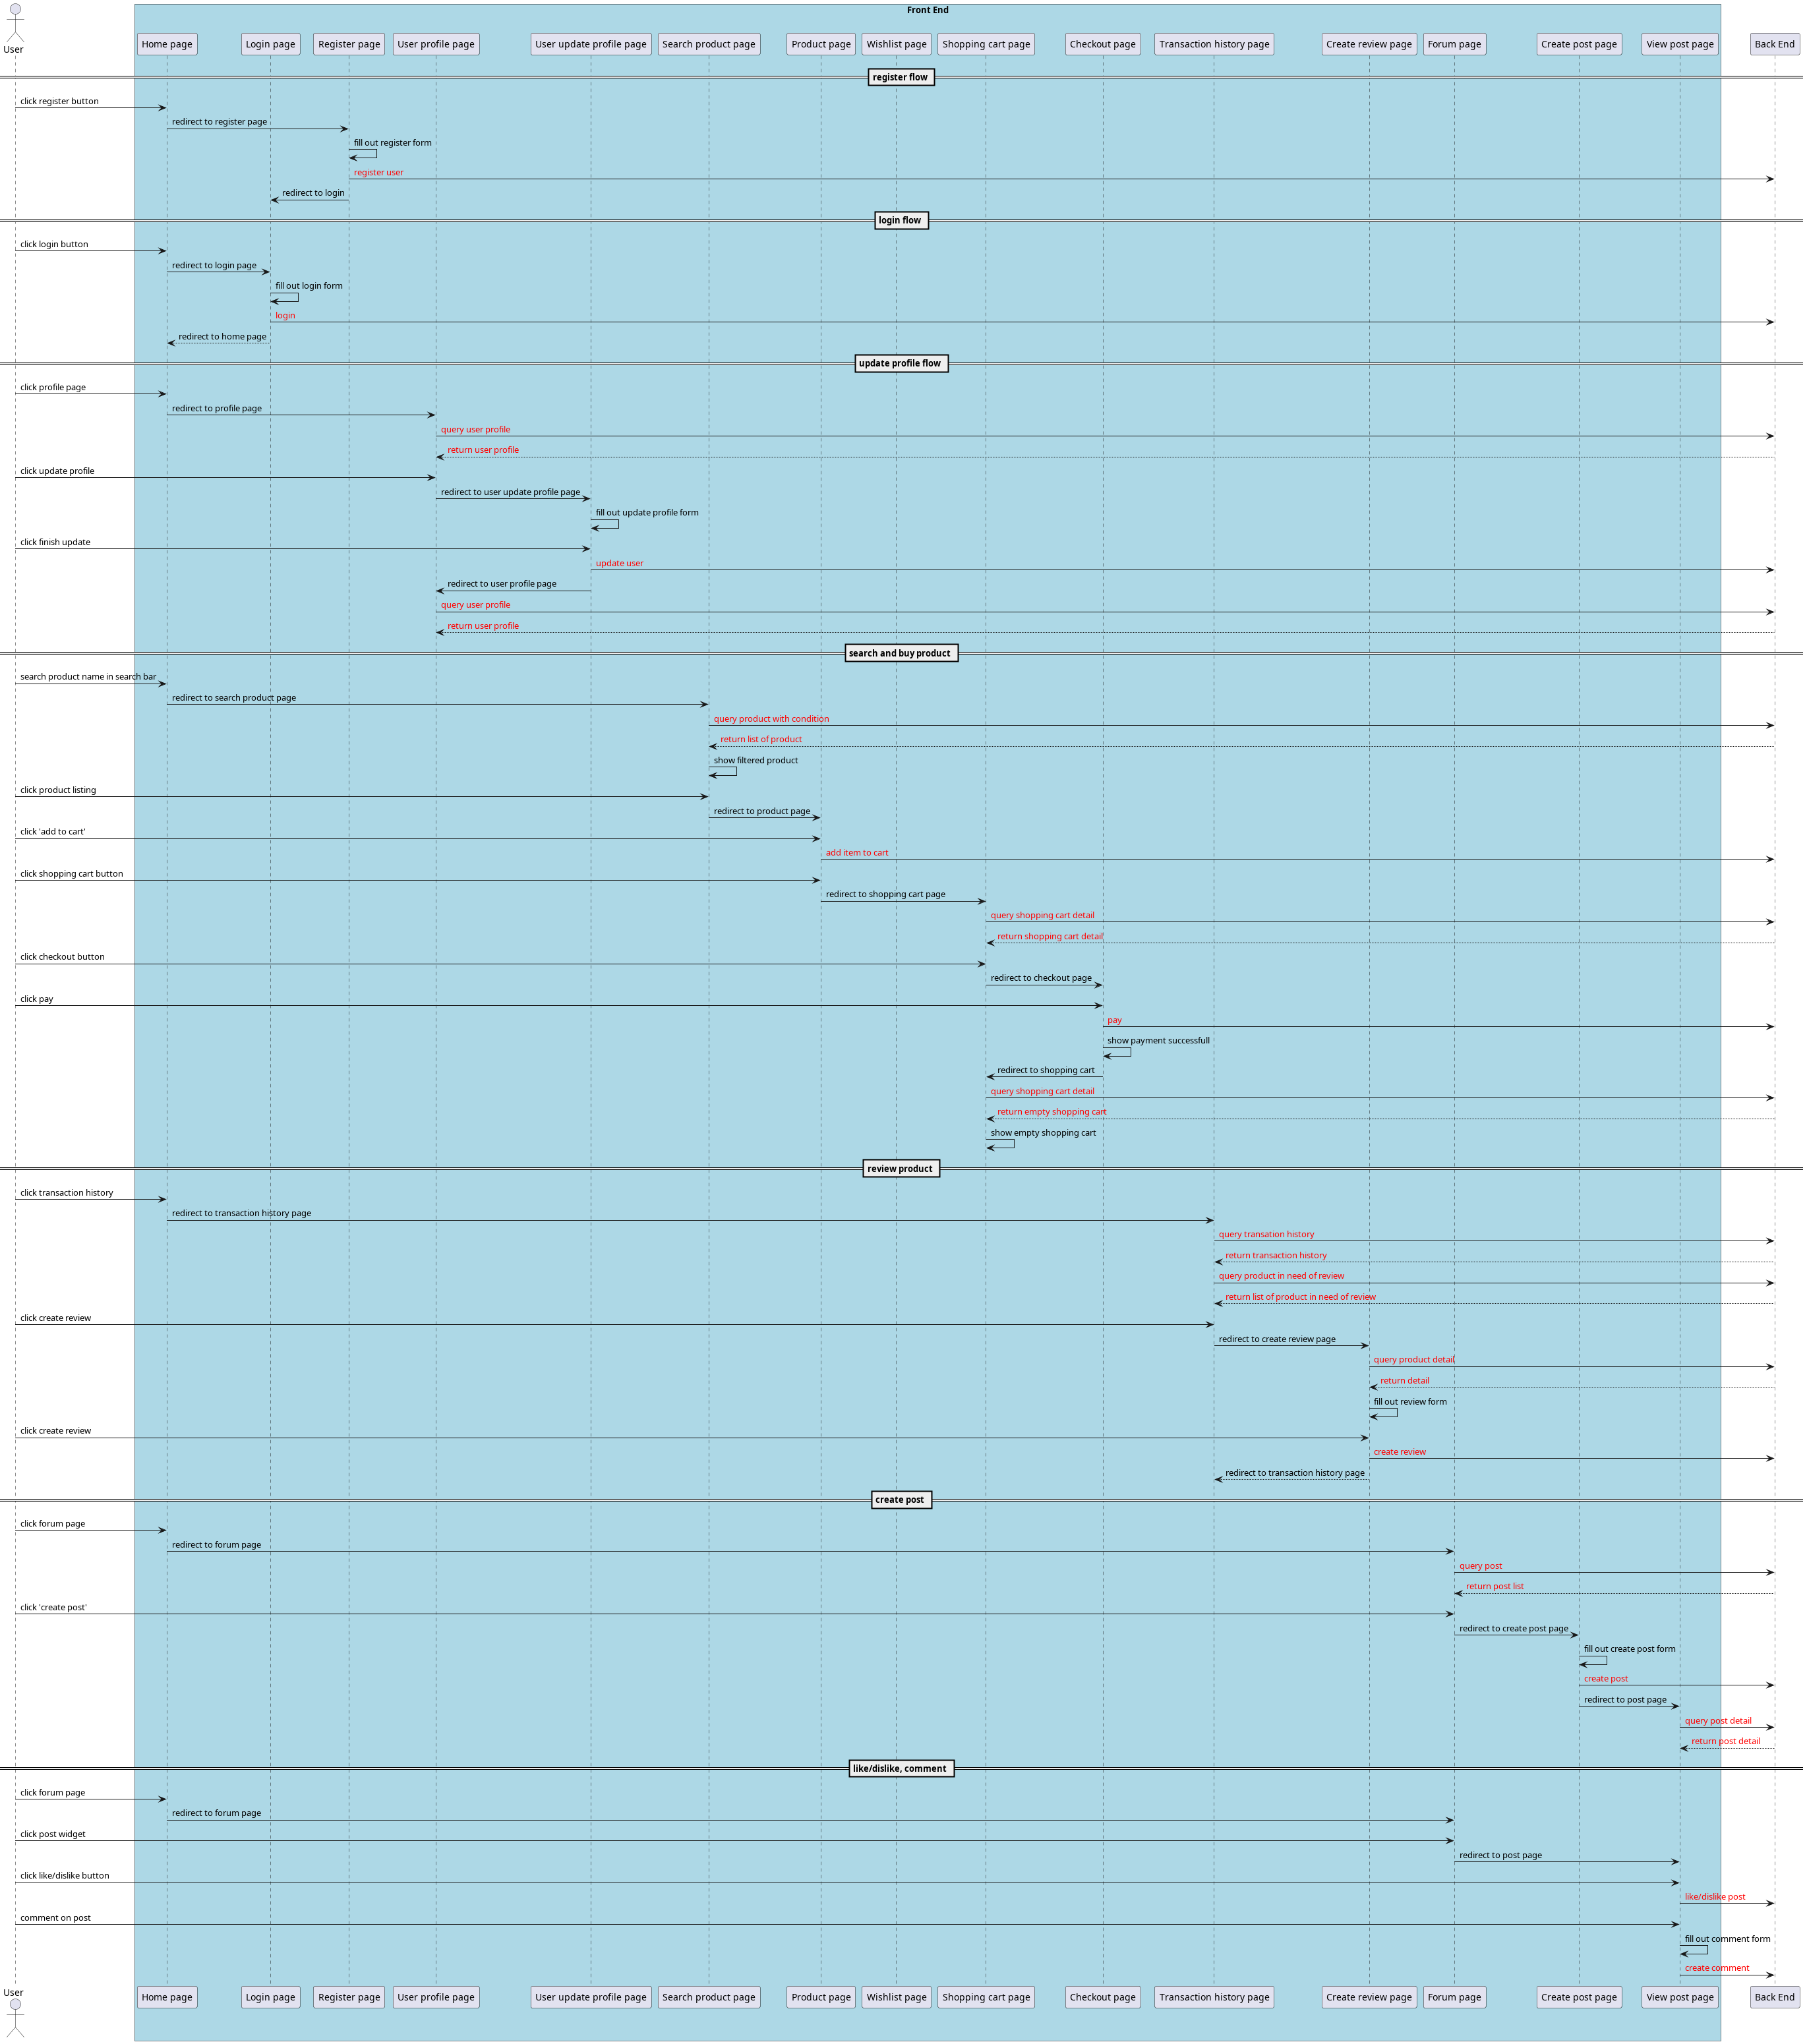
\includegraphics[height=12cm,keepaspectratio]{sequence diagram user perspective.png}
%                 \centering
%                 \caption{\textit{Sequence diagram} dari perspektif pembeli}
%             \end{figure}
%         \newpage
%         \item \textit{Merchant flow sequence diagram}
%             \begin{figure}[h]
%                 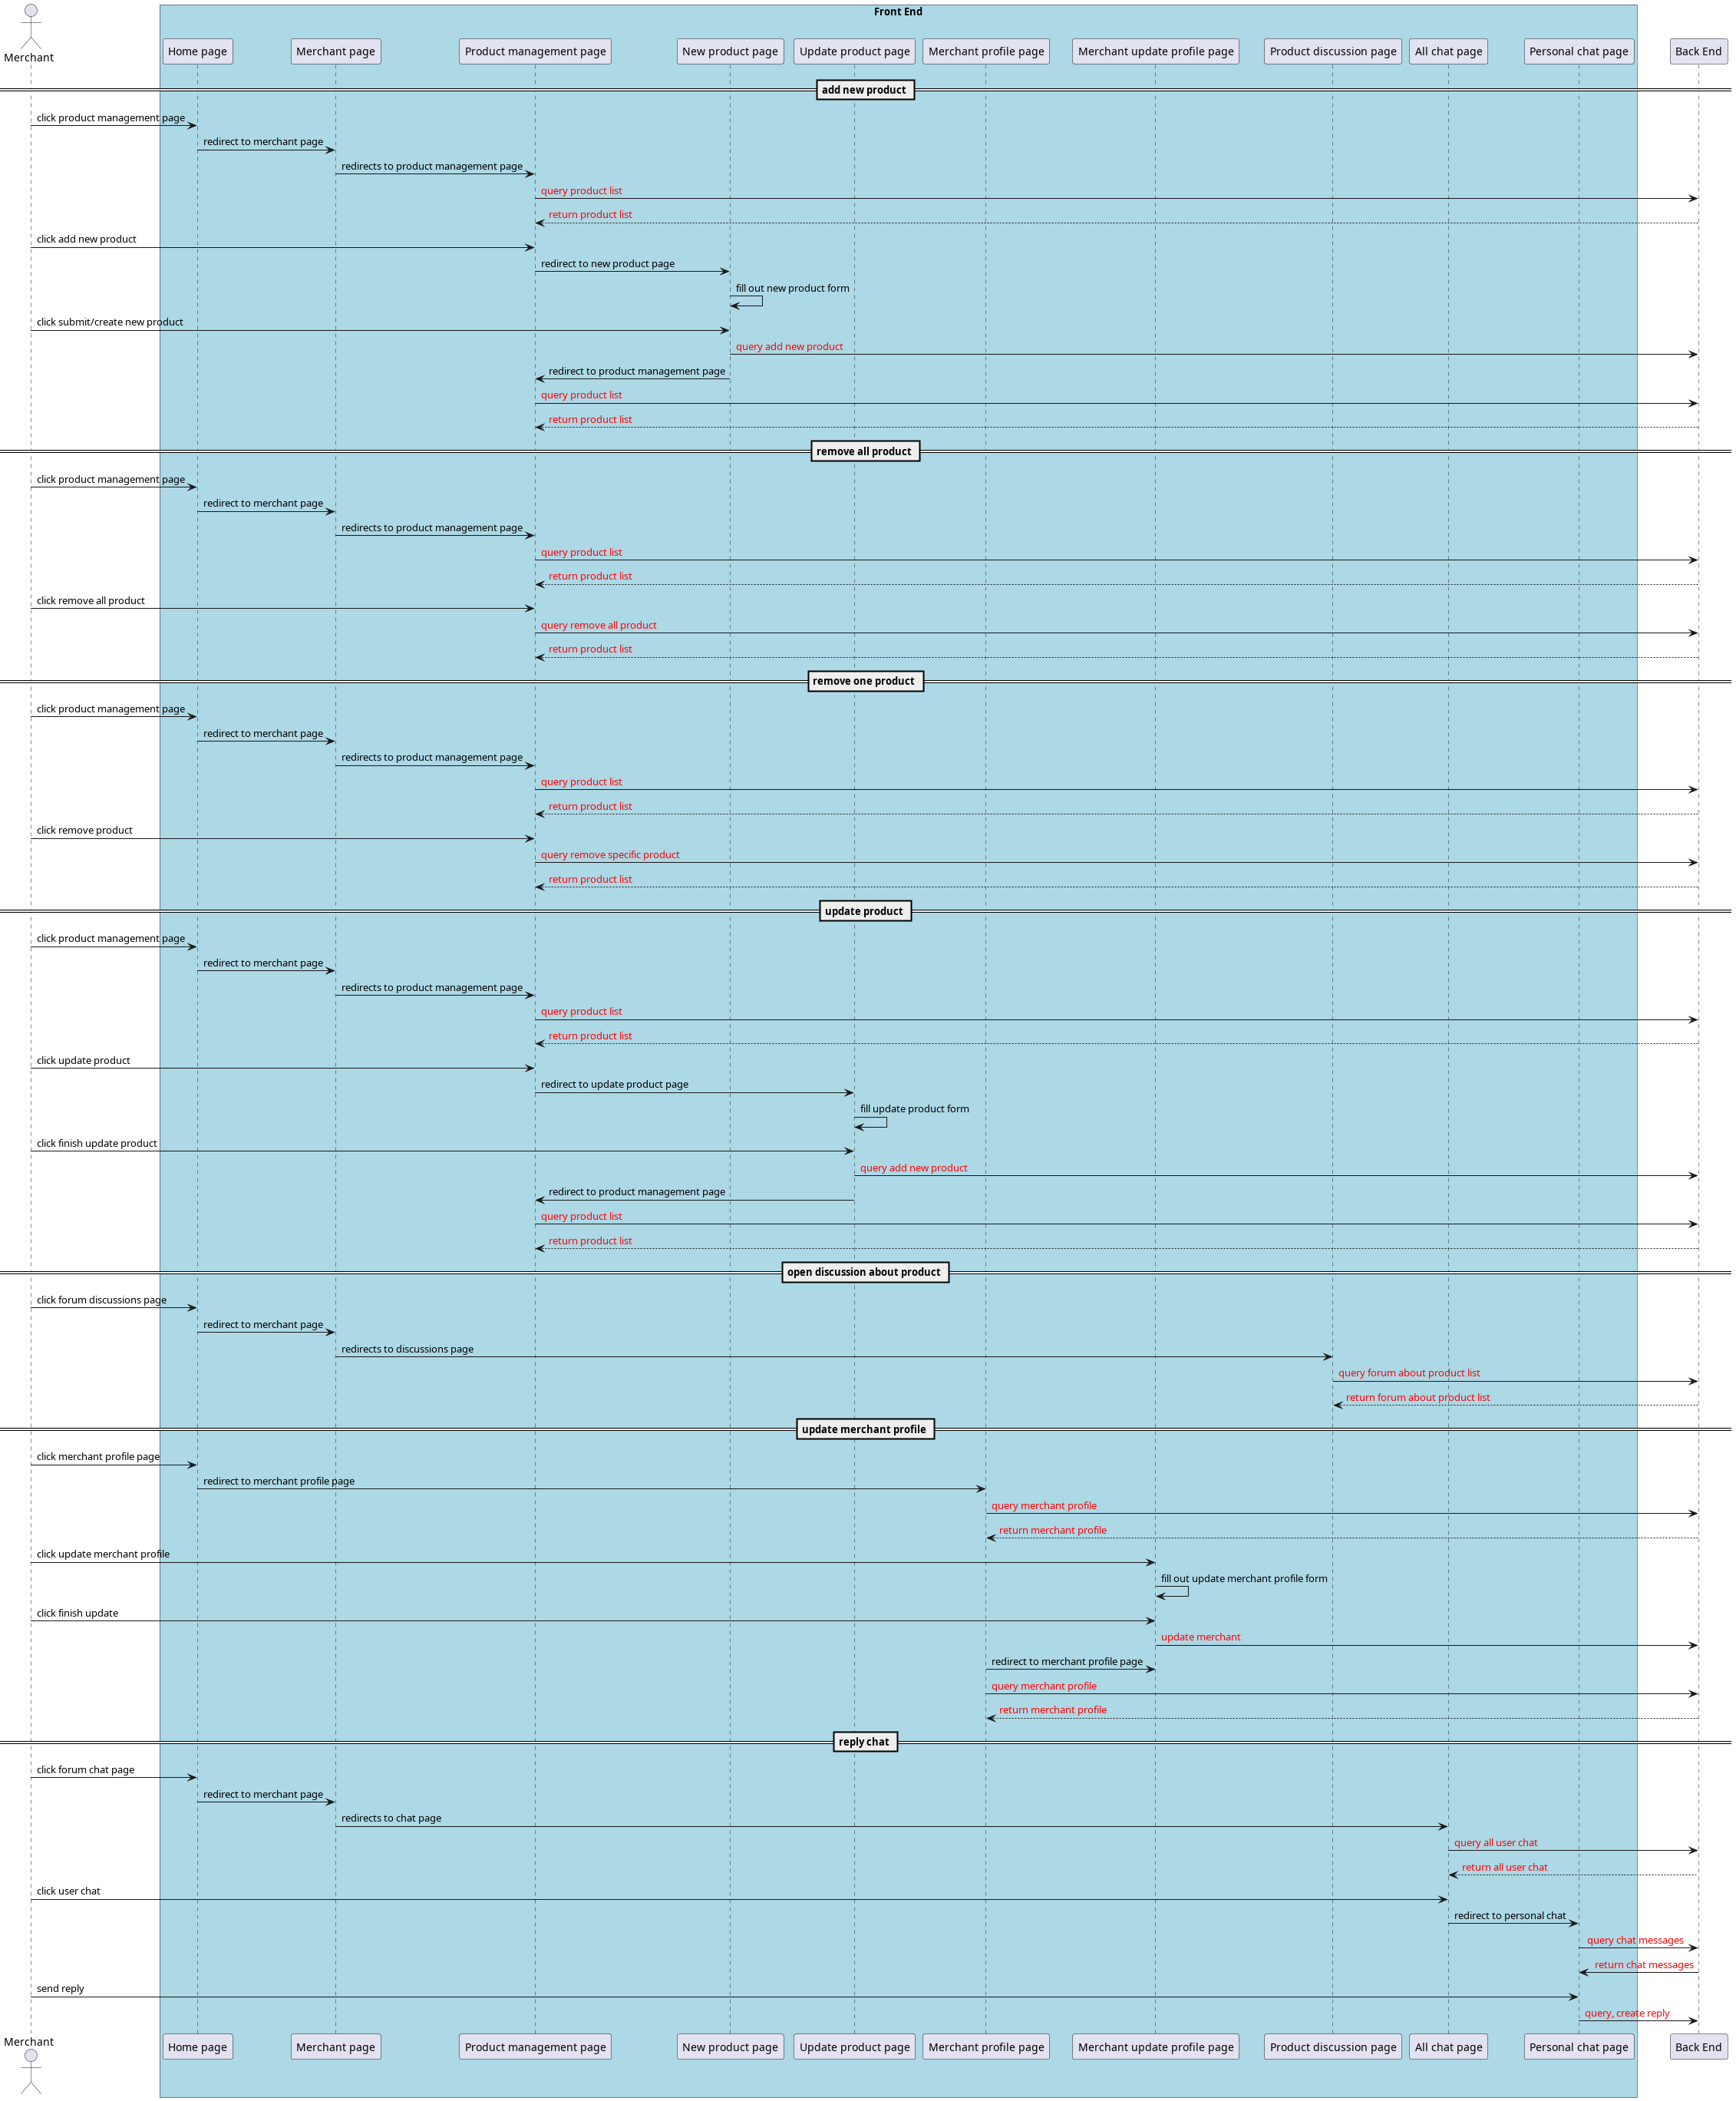
\includegraphics[height=12cm,keepaspectratio]{sequence diagram merchant perspective.png}
%                 \centering
%                 \caption{\textit{Sequence diagram} dari perspektif penjual}
%             \end{figure}
%         \newpage
%         \item \textit{Admin flow sequence diagram}
%             \begin{figure}[h]
%                 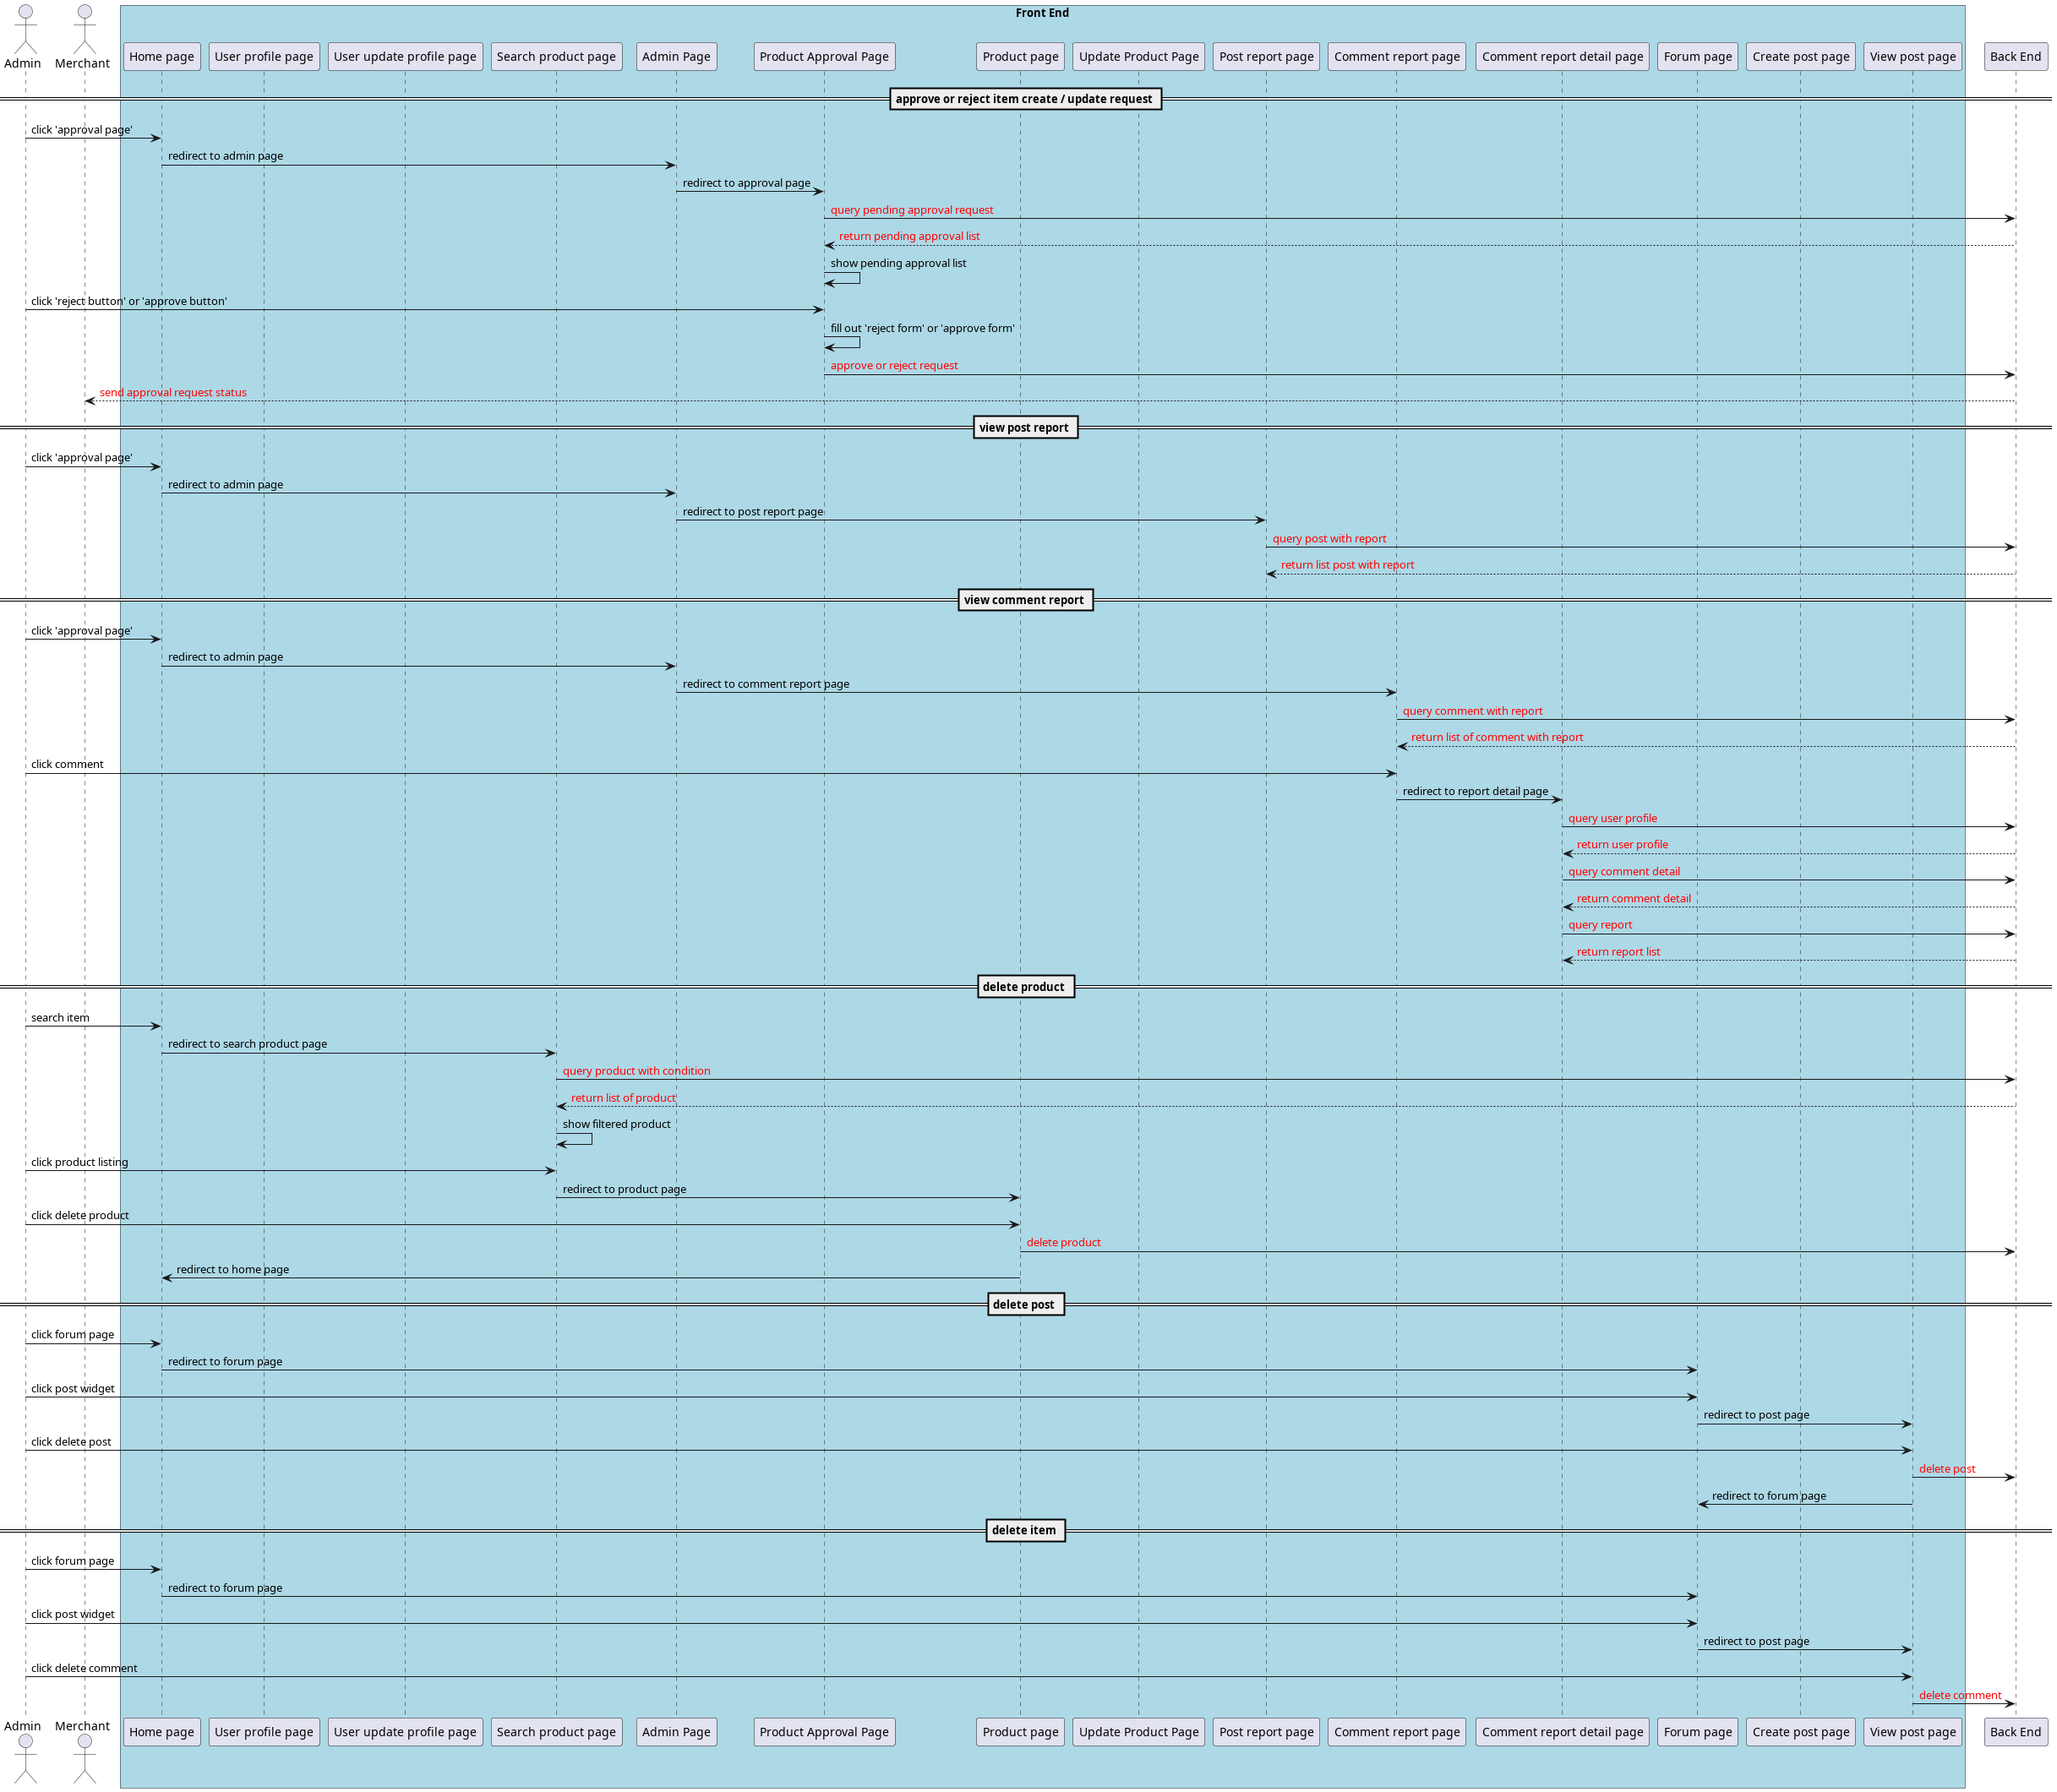
\includegraphics[height=12cm,keepaspectratio]{sequence diagram admin perspective.png}
%                 \centering
%                 \caption{\textit{Sequence diagram} dari perspektif \textit{admin}}
%             \end{figure}
%     \end{itemize}
% \end{enumerate}

\newpage
\addcontentsline{toc}{section}{\protect\numberline{}Referensi}
\printbibliography[title=Referensi]

\end{document}
